\documentclass[UTF8, fontset=ubuntu, oneside]{ctexbook}
\usepackage{parskip}
\usepackage{amsmath}
\usepackage{amssymb}
\usepackage{array}
\usepackage{graphicx}
\usepackage{float}
\usepackage{tikz}
\usepackage[framed]{ntheorem}
\usepackage{framed}
\usepackage[integrals]{wasysym}
\usetikzlibrary{datavisualization.formats.functions}
\newcommand*{\dif}{\mathop{}\!\mathrm{d}}
\renewcommand{\theequation}{\roman{equation}}
\renewcommand{\baselinestretch}{1.8}
\theoremstyle{empty}
\theoremheaderfont{\heiti}
\newframedtheorem{theorem}{定理}
\graphicspath{{./picture/}}
\def\mytypesetter#1{%
\pgfmathparse{#1/pi}%
\pgfmathprintnumber{\pgfmathresult}$\pi$%
}
\begin{document}
\chapter{方法、图像和直线}
1.函数\\
\textbf{函数}是将一个对象转化为另一个对象的规则. 起始对象称为\textbf{输入}, 来自称为\textbf{定义域}的集合. 返回对象称为\textbf{输出}, 来自称为\textbf{上域}的集合.

一个函数必须给每一个有效的输入指定唯一的输出.

\textbf{值域}是所有可能的输出所组成的集合.

\textbf{例1}.\\
$f(x)=x^2(x\in\mathbb{R}, f(x)\in\mathbb{R})$\\
在该示例中, 定义域为$\mathbb{R}$, 值域为$\mathbb{R}^+$, 上域为$\mathbb{R}$

区间定义:\\
$[a,b]$表示所有介于$a$和$b$ 之间(包括$a$和$b$)的实数的集合, 称为\textbf{闭区间}.\\
$(a,b)$表示所有介于$a$和$b$之间(不包括$a$和$b$)的实数的集合, 称为\textbf{开区间}.\\
$[a,b)$表示所有介于$a$和$b$之间(包括$a$, 不包括$b$)的实数的集合, 称为\textbf{半开区间}.

注意事项:\\
(1)分数的分母不能是零.\\
(2)不能取负数的偶次方根.\\
(3)不能取负数或零的对数.

垂线检验: 当任何一条垂直线与图像相交多于一次时, 该图像不是函数; 反之则图像为函数\\[2ex]

2.反函数\\
反函数的条件:\\
1)从一个函数$f$出发, 使得对于在$f$值域中的任意$y$, 都只有唯一的$x$值满足$f(x)=y$;\\
2)$f^{-1}$的定义域和$f$的值域相同;\\
3)$f^{-1}$的值域和$f$的定义域相同;\\
4)$f^{-1}(y)$的值就是满足$f(x)=y$的$x$. 即
\[\text{如果}\ f(x)=y, \text{则}\ f^{-1}(y)=x\]

水平线检验: 如果每一条水平线和一个函数的图像相交至多一次, 那么这个函数有反函数; 如果即使只有一条水平线和函数的图像相交多余一次, 那么这个函数没有反函数.

原始函数与反函数关于$y=x$对称

对于反函数, 有如下规则:\\
1)对于$f$值域中的所有$y$, 都有$f(f^{-1}(y))=y$;\\
2)对于$f$定义域中的$x$, 只有当$f$满足水平线检验时, 才有$f^{-1}(f(x))=x$.

例.\\
\phantom{例}$f(x)=\sin(x), \text{求}f^{-1}(f(x))$\\
推导过程:\\
当$f(x)$满足水平线检验时, $x\in[-\frac{\pi}{2},\frac{\pi}{2}]$\\
此时$f^{-1}(f(x))=x$\\[2ex]

3.复合函数\\
令$g(x)=x^2, h(x)=\cos(x)$, 而$f(x)=\cos(x^2)$, 则$f(x)=h(g(x))$, 也可表示为$f=h\circ g$, $f$为$g$与$h$的\textbf{复合函数}.\\[2ex]

4.奇函数与偶函数\\
如果$f$对定义域内的所有$x$有$f(-x)=f(x)$, 则$f$为\textbf{偶函数}.\\
如果$f$对定义域内的所有$x$有$f(-x)=-f(x)$, 则$f$为\textbf{奇函数}.

偶函数的图像关于y轴具有镜面对称性.\\
奇函数的图像关于原点有$180^o$的点对称性.\\[2ex]

5.线性函数\\
形如$f(x)=mx+b$的函数叫做\textbf{线性函数}.

点斜式方程:
\begin{center}
\begin{boxedminipage}{\textwidth}
	如果已知直线通过点$(x_0,y_0)$, 斜率为$m$, 则它的方程为$y-y_0=m(x-x_0)$
\end{boxedminipage}
\end{center}\vspace{4ex}

\begin{center}
\begin{boxedminipage}{11cm}
	如果一条直线通过点$(x_1,y_1)$和$(x_2,y_2)$, 则它的斜率等于$\displaystyle\frac{y_2-y_1}{x_2-x_1}$
\end{boxedminipage}
\end{center}\vspace{8ex}

6.常见函数\\
1)多项式\\
形如$f(x)=5x^4-4x^3+10$的函数\\[1ex]
基本项$x^n$的倍数叫做$x^n$的\textbf{系数}\\[1ex]
最大的幂指数$n$(该项系数不能为零)叫做多项式的\textbf{次数}\\[1ex]
最高次数项的系数称为\textbf{首项系数}\\

2)有理函数\\
形如$\displaystyle\frac{p(x)}{q(x)}$, 其中$p$和$q$为多项式\\

3)指数函数和对数函数\\
形如$y=a^x$的函数, 称为指数函数\\[1ex]
形如$\log_a(x)$的函数, 称为对数函数\\

4)带有绝对值的函数\\
\begin{center}
\begin{boxedminipage}{5cm}
\[|x|=\left\{
	\begin{array}{r l}
			x & \text{if}\ x\geqslant0\\
			-x & \text{if}\ x<0
	\end{array}
\right.\]
\end{boxedminipage}
\end{center}

%最后编辑于: 2022-01-19

\chapter{三角学回顾}
如图.\\
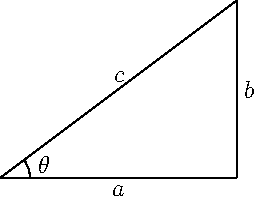
\includegraphics{triangel.pdf}

基本公式列表:\\
\begin{equation*}
\begin{array}{l l l}
    \displaystyle\sin(\theta)=\frac{b}{c} & \displaystyle\cos(\theta)=\frac{a}{c} & \displaystyle\tan(\theta)=\frac{b}{a}\\
    \displaystyle\csc(\theta)=\frac{1}{\sin(\theta)}=\frac{c}{b} & \displaystyle\sec(\theta)=\frac{1}{\cos(\theta)}=\frac{c}{a} & \displaystyle\cot(\theta)=\frac{1}{\tan(\theta)}=\frac{a}{b}
\end{array}
\end{equation*}
常见三角函数值:
\begin{equation*}
\begin{array}{>{\displaystyle}c|>{\displaystyle}c >{\displaystyle}c >{\displaystyle}c >{\displaystyle}c >{\displaystyle}c}
\hline
    & 0 & \frac{\pi}{6} & \frac{\pi}{4} & \frac{\pi}{3} & \frac{\pi}{2}\\[1ex]
\hline
    \sin & 0 & \frac{1}{2} & \frac{\sqrt{2}}{2} & \frac{\sqrt{3}}{2} & 1\\[1ex]
    \cos & 1 & \frac{\sqrt{3}}{2} & \frac{\sqrt{2}}{2} & \frac{1}{2} & 0\\[1ex]
    \tan & 0 & \frac{\sqrt{3}}{3} & 1 & \sqrt{3} & \star\\[1ex]
\hline
\end{array}
\end{equation*}

求三角函数值步骤:\\
1.找出角所在象限;\\
2.当角在x/y轴上, 参考三角函数图像;\\
3.如果角不在x/y轴上, 找出该角与x轴形成的最小角度, 即\textbf{参考角};\\
4.当参考角为特殊角时,参考常见三角函数值表;\\
5.利用ASTC(all/sin/tan/cos)决定是否需要添加负号.

三角函数图像:\\
\begin{figure}[H]
\centering
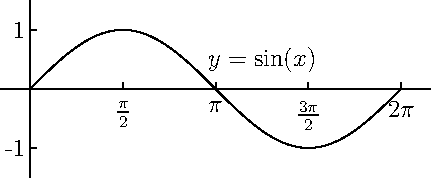
\includegraphics{sin.pdf}
\end{figure}
\begin{figure}
\centering
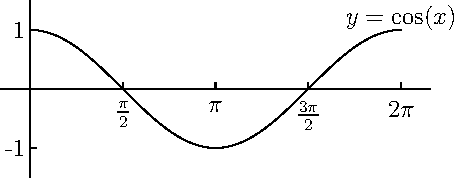
\includegraphics{cos.pdf}
\end{figure}
\begin{figure}
\centering
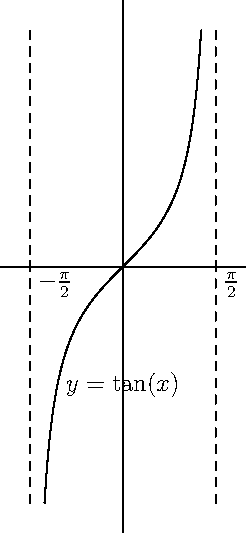
\includegraphics{tan.pdf}\qquad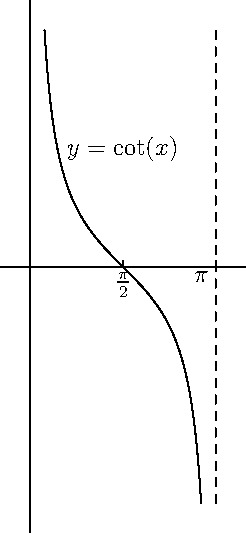
\includegraphics{cot.pdf}
\end{figure}
\begin{figure}
\centering
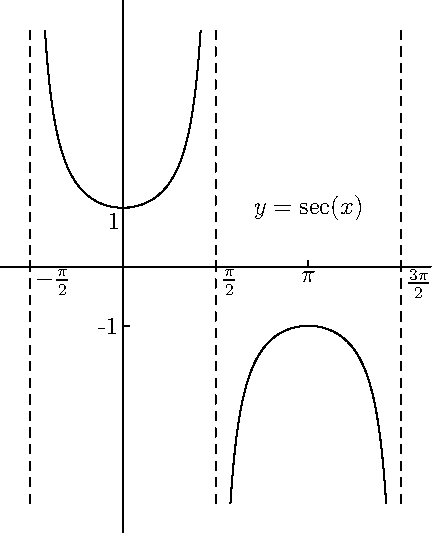
\includegraphics{sec.pdf}
\end{figure}
\begin{figure}
\centering
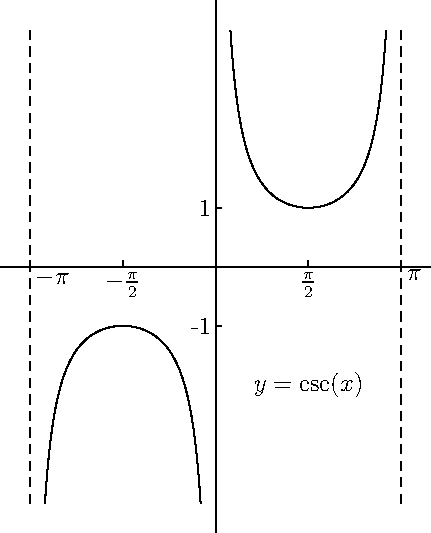
\includegraphics{csc.pdf}
\end{figure}

毕达哥拉斯定理:\\[-4ex]
\begin{center}
    \framebox{$\cos^2(x)+\sin^2(x)=1$}
\end{center}\vspace{4ex}

等式两边除以$\cos^2(x)$:\\[-4ex]
\begin{center}
    \framebox{$1+\tan^2(x)=\sec^2(x)$}
\end{center}\vspace{4ex}

等式两边除以$\sin^2(x)$:\\[-4ex]
\begin{center}
    \framebox{$\cot^2(x)+1=\csc^2(x)$}
\end{center}\vspace{4ex}

余角公式:\\[-4ex]
\begin{center}
    \framebox{$\cos(x)=\sin(\frac{\pi}{2}-x)$,$\cot(x)=\tan(\frac{\pi}{2}-x)$,$\csc(x)=\sec(\frac{\pi}{2}-x)$}\\[2ex]
    \framebox{$\sin(x)=\cos(\frac{\pi}{2}-x)$,$\tan(x)=\cot(\frac{\pi}{2}-x)$,$\sec(x)=\csc(\frac{\pi}{2}-x)$}
\end{center}\vspace{4ex}

和/差角公式:\\[-4ex]
\begin{center}
    \framebox{$\sin(A+B)=\sin(A)\cos(B)+\cos(A)\sin(B)$}\\[2ex]
    \framebox{$\cos(A+B)=\cos(A)\cos(B)-\sin(A)\sin(B)$}\\[2ex]
    \framebox{$\sin(A-B)=\sin(A)\cos(B)-\cos(A)\sin(B)$}\\[2ex]
    \framebox{$\cos(A-B)=\cos(A)\cos(B)+\sin(A)\sin(B)$}
\end{center}\vspace{4ex}

倍角公式:\\[-4ex]
\begin{center}
    \framebox{$\sin(2x)=2\sin(x)\cos(x)$}\\[2ex]
    \framebox{$\cos(2x)=\cos^2(x)-\sin^2(x)=2\cos^2(x)-1=1-2\sin^2(x)$}
\end{center}\vspace{8ex}

\chapter{极限导论}
极限: 描述函数的自变量接近于某一个值时, 相对应的函数值变化的趋势. 表示为:
\[\lim_{x\to a}f(x)=L\]\\[1em]
左极限: 描述函数的自变量从左边接近于某一个值时, 相对应的函数变化的趋势. 表示为
\[\lim_{x\to a^-}f(x)=L\]\\[1em]
右极限: 描述函数的自变量从右边接近于某一个值时, 相对应的函数变化的趋势. 表示为
\[\lim_{x\to a^+}f(x)=L\]\\[1em]
当左极限与右极限不相等时, 不存在双侧极限.\\[1em]
\begin{center}
\framebox{
\begin{minipage}{10cm}
``$f$在$x=a$处有一条垂直渐近线''说的是, $\displaystyle\lim_{x\to a^+}f(x)$和$\displaystyle\lim_{x\to a^-}f(x)$, 其中至少有一个极限是$\infty$或-$\infty$
\end{minipage}}
\end{center}\vspace{2em}
\begin{center}
\framebox{
\begin{minipage}{11cm}
``$f$在$y=L$处有一条右侧水平渐近线''意味着$\displaystyle\lim_{x\to\infty}f(x)=L$.\\
``$f$在$y=M$处有一条左侧水平渐近线''意味着$\displaystyle\lim_{x\to -\infty}f(x)=M$.
\end{minipage}}
\end{center}\vspace{2em}
三明治定理(夹逼定理):\\
\begin{center}
\framebox{
\begin{minipage}{10cm}
如果对于所有在$a$附近的$x$都有$g(x)\leqslant f(x)\leqslant h(x)$, 且$\displaystyle\lim_{x\to a}g(x)=\lim_{x\to a}h(x)=L$, 则$\displaystyle\lim_{x\to a}f(x)=L$.
\end{minipage}}
\end{center}

\chapter{求解多项式的极限问题}
1.$x\to a$时的有理函数的极限\\
有理函数: 形如$f(x)=\frac{p(x)}{q(x)}$的函数, 其中$p(x),q(x)$都是多项式.\\
1)当$f(a)=\frac{p(a)}{q(a)}=\frac{m}{n}$时:\\
$\displaystyle\lim_{x\to a}f(x)=\frac{m}{n}$\\
例.
\[\lim_{x\to -1}\frac{x^2-9}{x-2}=\lim_{x\to -1}\frac{x-9}{x-2}=\frac{1-9}{1-2}=8\]

2)当$f(a)=\frac{p(a)}{q(a)}=\frac{0}{0}$时:\\
$\displaystyle\lim_{x\to a}f(x)$进行分子分母约分\\
例.\\
\[\lim_{x\to 2}\frac{x^2-3x+2}{x-2}=\lim_{x\to 2}\frac{(x-1)(x-2)}{x-2}=\lim{x\to 2}x-1=2-1=1\]

3)当$f(a)=\frac{p(a)}{q(a)}=\frac{m}{0}$时:\\
$\displaystyle\lim_{x\to a}f(x)$判断极限点两边的极限是否同为$\infty$或$-\infty$\\
例.\\
$\displaystyle\lim_{x\to 1}\frac{2x^2-x-6}{x(x-1)^3}=\lim_{x\to 1}\frac{(2x+3)(x-2)}{x(x-1)^3}$\\
$\displaystyle\mathbf{\because}\lim_{x\to 1^-}\frac{(2x+3)(x-2)}{x(x-1)^3}=\frac{(+)(-)}{(+)(-)}=+$\\
$\displaystyle\phantom{\because}\lim_{x\to 1^+}\frac{(2x+3)(x-2)}{x(x-1)^3}=\frac{(+)(-)}{(+)(+)}=-$\\
$\displaystyle\mathbf{\therefore}\,f(x)\text{无极限值}$\\[2ex]

2.$x\to a$时的平方根的极限\\
共轭因式: 若S是含有根式的已知表达式, 若存在一个不恒等于零的表达式M, 使乘积S$\times$M不含根式, 则M为S的共轭因式. 反之, S也为M的共轭因式.\\
设$f(x)=\frac{g(x)\pm h(x)}{p(x)\pm q(x)}$, 其中, g(x)/h(x)/p(x)/q(x)其中一个为根式\\
当$f(a)=\frac{g(a)-h(a)}{p(a)-q(a)}=\frac{0}{0}$时, 将分子分母同时乘以含根号部分的共轭因式.\\
例.
\begin{displaymath}
\begin{array}{l}
    \displaystyle\lim_{x\to 5}\frac{\sqrt{x^2-9}-4}{x-5}=\lim_{x\to 5}\frac{\sqrt{x^2-9}-4}{x-5}\times\frac{\sqrt{x^2-9}+4}{\sqrt{x^2-9}+4}=\lim_{x\to 5}\frac{x^2-25}{(x-5)(\sqrt{x^2-9}+4)}\\
    \displaystyle\phantom{\lim_{x\to 5}\frac{\sqrt{x^2-9}-4}{x-5}}=\lim_{x\to 5}\frac{x+5}{\sqrt{x^-9}+4}=\frac{5+5}{\sqrt{25-9}+4}=\frac{5}{4}
\end{array}
\end{displaymath}\vspace{2ex}

3.$x\to\infty/-\infty$时的有理函数的极限\\
\begin{math}
\begin{array}{l}
	\because\displaystyle\lim_{x\to\infty}\frac{C}{x^n}=0\\
	\therefore\displaystyle\lim_{x\to\infty}f(x)=\lim_{x\to\infty}\frac{p(x)}{q(x)}=\lim_{x\to\infty}\frac{a_{0}x^m+a_{1}x^{m-1}+\cdots+a_{m}}{b_{0}x^n+b_{1}x^{n-1}+\cdots+b_{n}}\\
	\displaystyle\phantom{\therefore\lim_{x\to\infty}f(x)}=\lim_{x\to\infty}\frac{\frac{a_{0}x^m+a_{1}x^{m-1}+\cdots+a_{m}}{a_{0}x^m}\times a_{0}x^m}{\frac{b_{0}x^n+b_{1}x^{n-1}+\cdots+b_{n}}{b_{0}x^n}\times b_{0}x^n}\\
	\displaystyle\phantom{\therefore\lim_{x\to\infty}f(x)}=\lim_{x\to\infty}\frac{a_{0}x^m}{b_{0}x^n}\\
	\displaystyle\phantom{\therefore\lim_{x\to\infty}f(x)}=\frac{a_0}{b_0}\lim_{x\to\infty}\frac{x^m}{x^n}
\end{array}\\[1ex]
\end{math}
情况分布:\\
(1)m=n, 极限为有限的且非零;\\
(2)m>n, 极限为$\infty$或$-\infty$;\\
(3)m<n, 极限为0.\\[2ex]

4.$x\to\infty$时的多项式型函数的极限\\
\begin{math}
\begin{array}{l}
	\displaystyle\lim_{x\to\infty}f(x)=\lim_{x\to\infty}\frac{p(x)}{q(x)}=\lim_{x\to\infty}\frac{\sqrt{a_{0}x^m+a_{1}x^{m-1}+\cdots+a_{m}}}{b_{0}x^n+b_{1}x^{n-1}+\cdots+b_{n}}\\
	\displaystyle\phantom{\lim_{x\to\infty}f(x)}=\lim_{x\to\infty}\frac{\frac{\sqrt{a_{0}x^m+a_{1}x^{m-1}+\cdots+a_{m}}}{\sqrt{a_0}x^{\frac{m}{2}}}\times\sqrt{a_0}x^{\frac{m}{2}}}{\frac{b_{0}x^n+b_{1}x^{n-1}+\cdots+b_{n}}{b_{0}x^n}\times b_{0}x^n}\\
	\displaystyle\phantom{\lim_{x\to\infty}f(x)}=\lim_{x\to\infty}\frac{\sqrt{a_0}x^{\frac{m}{2}}}{b_{0}x^n}\\
	\displaystyle\phantom{\lim_{x\to\infty}f(x)}=\frac{\sqrt{a_0}}{b_0}\lim_{x\to\infty}\frac{x^{\frac{m}{2}}}{x^n}
\end{array}
\end{math}\\[2ex]

5.$x\to-\infty$时的多项式型函数的极限\\
与类型4类似. 但有一种特殊情况:\\[1ex]
\framebox{
\begin{minipage}[c]{10cm}
    如果$x<0$, 并且$\sqrt[n]{x^p}=x^m$, 那么需要在$x^m$之前加一个负号的唯一情形是: n是偶的而m是奇的.
\end{minipage}
}\\[2ex]

6.包含绝对值的函数的极限\\
\begin{math}
\begin{array}{l}
\because p(x)>0, |p(x)|=p(x)\\ 
\phantom{\because}p(x)<0, |p(x)|=-p(x)\\
\displaystyle\therefore\lim_{x\to -2^-}\frac{|x+2|}{x+2}=\frac{-(x+2)}{x+2}=-1\\
\displaystyle\phantom{\therefore}\lim_{x\to -2^+}\frac{|x+2|}{x+2}=\frac{x+2}{x+2}=1\\
\displaystyle\therefore\lim_{x\to -2}\frac{|x+2|}{x+2}\text{无双侧极限}
\end{array}
\end{math}

\documentclass[UFT8, fontset=ubuntu]{ctexart}
\usepackage{parskip}
\begin{document}
1.在一点处连续\\[1ex]
\framebox{如果$\displaystyle\lim_{x\to a}f(x)=f(a)$, 函数$f$在点$x=a$处连续}\\[4ex]
2.在区间上连续\\
在区间$(a,b)$上连续 - 函数在区间范围内的所有点都连续(不包括$a,b$)\\
在区间$[a,b]$上连续 - (1)函数在(a,b)上连续; (2)函数在$x=a$处右连续(即$\displaystyle\lim_{x\to a^+}=f(a)$); (3)函数在$x=b$处左连续(即$\displaystyle\lim_{x\to a^-}=f(b)$)\\[4ex]
\framebox{
\begin{minipage}[c]{12cm}
	\textbf{介值定理:}如果$f$在$[a,b]$上连续, 并且$f(a)<0$且$f(b)>0$, 那么在区间$(a,b)$上至少有一点$c$, 使得$f(c)=0$. 代之以$f(a)>0$且$f(b)<0$, 同样成立.
\end{minipage}}\\[4ex]
\framebox{
\begin{minipage}[c]{12cm}
	\textbf{最大值与最小值定理:}如果$f$在$[a,b]$上连续, 那么$f$在$[a,b]$上至少有一个最大值和一个最小值.
\end{minipage}}\\[4ex]
求导公式:
\[f'(x)=f^{(1)}(x)=\frac{dy}{dx}=\lim_{h\to 0}\frac{f(x+h)-f(x)}{h}\]
二阶及多阶导数:\\
\begin{math}
\begin{array}{l}
	\displaystyle f''(x)=f^{(2)}(x)=\frac{d^2y}{dx^2}\\[2ex]
	\displaystyle f'''(x)=f^{(3)}(x)=\frac{d^3y}{fx^3}\\[2ex]
	\cdots
\end{array}
\end{math}\\[2ex]
\framebox{如果一个函数$f$在$x$上可导, 那么它在$x$上连续}
\end{document}

\chapter{求解微分问题}
1.使用定义求导\\
\framebox{$\displaystyle\frac{\dif}{\dif x}(x)=1$}\\
证明:\\
$\displaystyle\lim_{h\to 0}\frac{f(x+h)-f(x)}{h}=\lim_{h\to 0}\frac{(x+h)-x}{h}=\lim_{h\to 0}\frac{h}{h}=1$\\[4ex]

\framebox{$\displaystyle\frac{\dif}{\dif x}(\sqrt{x})=\frac{1}{2\sqrt{x}}$}\\
证明:\\
\begin{math}
\begin{array}{l}
\displaystyle\lim_{h\to 0}\frac{f(x+h)-f(x)}{h}=\lim_{h\to 0}\frac{\sqrt{x+h}-\sqrt{x}}{h}=\lim_{h\to 0}\frac{\sqrt{x+h}-\sqrt{x}}{h}\times\frac{\sqrt{x+h}+\sqrt{x}}{\sqrt{x+h}+\sqrt{x}}\\
\displaystyle\phantom{\lim_{h\to 0}\frac{f(x+h)-f(x)}{h}}=\lim_{h\to 0}\frac{h}{h(\sqrt{x+h}+\sqrt{x})}=\lim_{h\to 0}\frac{1}{\sqrt{x+h}+\sqrt{x}}=\frac{1}{2\sqrt{x}}
\end{array}
\end{math}\\[4ex]

\framebox{$\displaystyle\frac{\dif}{\dif x}(\frac{1}{x})=-\frac{1}{x^2}$}\\
证明:\\
\begin{math}
\begin{array}{l}
\displaystyle\lim_{h\to 0}\frac{f(x+h)-f(x)}{h}=\lim_{h\to 0}\frac{\frac{1}{x+h}-\frac{1}{x}}{h}=\lim_{h\to 0}\frac{-\frac{h}{x(x+h)}}{h}\\
\displaystyle\phantom{\lim_{h\to 0}\frac{f(x+h)-f(x)}{h}}=\lim_{h\to 0}-\frac{1}{x(x+h)}=-\frac{1}{x^2}
\end{array}
\end{math}\\[4ex]

\framebox{$\displaystyle\frac{\dif}{\dif x}(x^a)=ax^{a-1}$}\\[4ex]

2.运算法则\\
(1)常数倍\\
$\displaystyle\frac{\dif}{\dif x}(Cx^a)=(Ca)x^{a-1}$\\[4ex]
(2)加/减法法则\\
$\displaystyle\frac{\dif}{\dif x}(x^a+\sqrt{x})=\frac{\dif}{\dif x}(x^a)+\frac{\dif}{\dif x}(\sqrt{x})$\\[4ex]
(3)乘积法则\\[-6ex]
{\par\centering
\framebox{\textbf{乘积法则(版本1)}\qquad 如果$h(x)=f(x)g(x)$, 那么$h'(x)=f'(x)g(x)+f(x)g'(x)$.}\\[2ex]
\framebox{
\begin{minipage}[c]{6cm}
\textbf{乘积法则(版本2)}\quad 如果$y=uv$, 则
\[\frac{\dif y}{\dif x}=v\frac{\dif u}{\dif x}+u\frac{\dif v}{\dif x}\]
\end{minipage}}\\[4ex]
\framebox{
\begin{minipage}[c]{7cm}
\textbf{乘积法则(三个变量)}\quad 如果$y=uvw$, 则
\[\frac{\dif y}{\dif x}=\frac{\dif u}{\dif x}vw+u\frac{\dif v}{\dif x}w+uv\frac{\dif w}{\dif x}\]
\end{minipage}}
\par}\vspace{4ex}
(4)商法则\\[-4ex]
{\par\centering
\framebox{
\begin{minipage}[c]{8cm}
\textbf{商法则(版本1)}\quad 如果$h(x)=\frac{f(x)}{g(x)}$, 那么
\[h'(x)=\frac{f'(x)g(x)-f(x)g'(x)}{(g(x))^2}\]
\end{minipage}}\\[2ex]
\framebox{
\begin{minipage}[c]{6cm}
\textbf{商法则(版本2)}\quad 如果$y=\frac{u}{v}$, 那么
\[\frac{\dif y}{\dif x}=\frac{v\frac{\dif u}{\dif x}-u\frac{\dif v}{\dif x}}{v^2}\]
\end{minipage}}
\par}\vspace{4ex}
(5)链式求导法则\\[-6ex]
{\par\centering
\framebox{\textbf{链式求导法则(版本1)}\quad 如果$h(x)=f(g(x))$, 那么$h'(x)=f'(g(x))g'(x)$.}\\[2ex]
\framebox{
\begin{minipage}[c]{12cm}
\textbf{链式求导法则(版本2)}\quad 如果$y$是$u$的函数, 并且$u$是$x$的函数, 那么
\[\frac{\dif y}{\dif x}=\frac{\dif y}{\dif u}\frac{\dif u}{\dif x}\]
\end{minipage}}
\par}\vspace{4ex}

3.导数伪装的极限\\
例.\\
$\displaystyle\lim_{h\to 0}\frac{\sqrt[5]{32+h}-2}{h}$\\
证明:\\
设$f(x)=\sqrt[5]{x}$\\
$\displaystyle\because f'(x)=\lim_{h\to 0}\frac{\sqrt[5]{x+h}-x}{h}=\frac{1}{5}x^{-\frac{4}{5}}$\\
$\displaystyle\therefore f'(32)=\lim_{h\to 0}\frac{\sqrt[5]{32+h}-\sqrt[5]{32}}{h}=\lim_{h\to 0}\frac{\sqrt[5]{32+h}-2}{h}=\frac{1}{5}\times 32^{-\frac{4}{5}}=\frac{1}{5}\times\frac{1}{16}=\frac{1}{80}$\\

4.分段函数的导数\\
检验方式: 分段函数再连接点上极限相等, 并且导数再连接点上的极限也相等\\
例.\\
$f(x)=\left\{
\begin{array}{l l}
1 & \text{如果}x\leqslant0,\\
x^2+1 & \text{如果}x>0.    
\end{array}
\right.$\\
$\because f(x)$在连接点$x=0$上的左极限:\\
$\phantom{\because}\displaystyle\lim_{x\to0^-}f(x)=\lim_{x\to0^-}1=1$\\
$\phantom{\because}f(x)$在连接点$x=0$上的右极限:\\
$\phantom{\because}\displaystyle\lim_{x\to0^+}f(x)=\lim_{x\to0^+}(x^2+1)=1$\\
$\therefore\displaystyle\lim_{x\to0}f(x)=1$\\[2ex]
由于, $f'(x)=\left\{
\begin{array}{l l}
	0 & \text{如果}x\leqslant 0,\\
	2x & \text{如果}x>0.
\end{array}
\right.$\\
$\because f'(x)$在连接点$x=0$上的左极限:\\
$\phantom{\because}\displaystyle\lim_{x\to0^-}f'(x)=\lim_{x\to0^-}0=0$\\
$\phantom{\because}f'(x)$在连接点$x=0$上的右极限:\\
$\phantom{\because}\displaystyle\lim_{x\to0^+}f'(x)=\lim_{x\to0^+}2x=0$\\
$\therefore\displaystyle\lim_{x\to0}f'(x)=0$\\

5.直接画出导函数的图像

\chapter{三角函数的极限和导数}
1.三角函数的极限:\\
(1)$x\to 0$的情况\\[2ex]
\framebox{$\displaystyle\lim_{x\to 0}\frac{\sin x}{x}=1$}\\[2ex]
\framebox{$\displaystyle\lim_{x\to 0}\frac{\tan x}{x}=1$}\\[2ex]
\framebox{$\displaystyle\lim_{x\to 0}\cos x=1$}\\[2ex]
\framebox{$\displaystyle\lim_{x\to 0}\frac{1-\cos x}{x}=0$}\\[2ex]
例1.\\
\phantom{例}$\displaystyle\lim_{x\to 0}\frac{\sin5x}{x}$\\
$\displaystyle\lim_{x\to 0}\frac{\sin5x}{x}=\lim_{x\to 0}\frac{\frac{\sin5x}{5x}}{x}\times5x=1\times5=5$\\

例2.\\
\phantom{例}$\displaystyle\lim_{x\to 0}\frac{\sin^3(2x)\cos(5x^{19})}{x\tan(5x^2)}$
$\displaystyle\lim_{x\to 0}\frac{\sin^3(2x)\cos(5x^{19})}{x\tan(5x^2)}=\lim_{x\to 0}\frac{[\frac{(\sin(2x))^3}{(2x)^3}\times (2x)^3]\cos(5x^{19})}{x[\frac{\tan(5x^2)}{5x^2}\times (5x^2)]}$\\
$\displaystyle\phantom{\lim_{x\to 0}\frac{\sin^3(2x)\cos(5x^{19})}{x\tan(5x^2)}}=\lim_{x\to 0}\frac{\frac{(\sin(2x))^3}{(2x)^3}\cdot\cos(5x^{19})}{\frac{\tan(5x^2)}{5x^2}}\times\frac{(2x)^3}{x(5x^2)}$\\
$\displaystyle\phantom{\lim_{x\to 0}\frac{\sin^3(2x)\cos(5x^{19})}{x\tan(5x^2)}}=\lim_{x\to 0}\frac{8x^3}{5x^3}$\\
$\displaystyle\phantom{\lim_{x\to 0}\frac{\sin^3(2x)\cos(5x^{19})}{x\tan(5x^2)}}=\frac{8}{5}$\\

例3.\\
\phantom{例}$\displaystyle\lim_{x\to 0}x\sin(\frac{5}{x})$\\
$\displaystyle\lim_{x\to 0}x\sin(\frac{5}{x})=\lim_{x\to 0}\frac{\sin(frac{5}{x})}{\frac{5}{x}}\times5=1\times5=5$\\

例4.\\
\phantom{例}$\displaystyle\lim_{x\to 0}\frac{1-\cos x}{x^2}$\\
$\displaystyle\lim_{x\to 0}\frac{1-\cos x}{x^2}=\lim_{x\to 0}\frac{1-\cos x}{x^2}\times\frac{1+\cos x}{1+\cos x}=\lim_{x\to 0}\frac{1-\cos^2x}{x^2(1+\cos x)}$\\
$\displaystyle\phantom{\lim_{x\to 0}\frac{1-\cos x}{x^2}}=\lim_{x\to 0}\frac{\sin^2x}{x^2}\times\frac{1}{1+\cos x}=1\times\frac{1}{2}=\frac{1}{2}$\\[2ex]

(2)$x\to\infty/-\infty$的情况\\
例.\\
\phantom{例}$\displaystyle\lim_{x\to\infty}\frac{x\sin(11x^7)-\frac{1}{2}}{2x^4}$\\
$\displaystyle\because-1\leqslant\sin(11x^7)\leqslant1$\\
$\displaystyle\therefore-x-\frac{1}{2}\leqslant x\sin(11x^7)-\frac{1}{2}\leqslant x-\frac{1}{2}$\\
$\displaystyle\phantom{\therefore}\frac{-x-\frac{1}{2}}{2x^4}\leqslant\frac{x\sin(11x^7)-\frac{1}{2}}{2x^4}\leqslant\frac{x-\frac{1}{2}}{2x^4}$\\
而$\displaystyle\lim_{x\to\infty}\frac{-x-\frac{1}{2}}{2x^4}=\lim_{x\to\infty}-\frac{1}{2x^3}-\frac{1}{4x^4}=0$\\
\phantom{而}$\displaystyle\lim_{x\to\infty}\frac{x-\frac{1}{2}}{2x^4}=\lim_{x\to\infty}\frac{1}{2x^3}-\frac{1}{4x^4}=0$\\
$\displaystyle\therefore$根据夹逼定理\\
$\displaystyle\phantom{\therefore}\lim_{x\to\infty}\frac{x\sin(11x^7)-\frac{1}{2}}{2x^4}=0$\\[2ex]

(3)其他情况\\
面对$x\to a$的极限, 而$a\neq 0$时, 使用$t=x-a$作替换, 将问题转化为$t\to 0$\\
例.\\
\phantom{例}$\displaystyle\lim_{x\to\frac{\pi}{2}}\frac{\cos x}{x-\frac{\pi}{2}}$\\
设$t=x-\frac{\pi}{2}$, 则\\
$\displaystyle\lim_{x\to\frac{\pi}{2}}\frac{\cos x}{x-\frac{\pi}{2}}=\lim_{t\to 0}\frac{\cos(t+\frac{\pi}{2})}{t}$\\
$\displaystyle\because\cos(\frac{\pi}{2}-x)=\sin x$\\
$\displaystyle\therefore\cos(\frac{\pi}{2}+x)=\sin(-x)=-\sin x$\\
$\displaystyle\therefore\lim_{t\to 0}\frac{\cos(t+\frac{\pi}{2})}{t}=\lim_{t\to 0}\frac{-\sin t}{t}=-1$\\[2ex]

2.三角函数的导数\\[2ex]
\framebox{$\displaystyle\frac{\dif}{\dif x}\sin(x)=\cos(x)$}\\[2ex]
\framebox{$\displaystyle\frac{\dif}{\dif x}\cos(x)=-\sin(x)$}\\[2ex]
\framebox{$\displaystyle\frac{\dif}{\dif x}\tan(x)=\sec^2(x)$}\\[2ex]
\framebox{$\displaystyle\frac{\dif}{\dif x}\cot(x)=-\csc^2(x)$}\\[2ex]
\framebox{$\displaystyle\frac{\dif}{\dif x}\sec(x)=\sec(x)\tan(x)$}\\[2ex]
\framebox{$\displaystyle\frac{\dif}{\dif x}\csc(x)=-\csc(x)\cot(x)$}\\[2ex]

例1.\\
\phantom{例}$\displaystyle\frac{\dif}{\dif x}x^2\sin x$\\
根据乘积法则:\\
$u=x^2$, $v=\sin x$\\
$\frac{\dif u}{\dif x}=2x$, $\frac{\dif v}{\dif x}=\cos x$\\
$\frac{\dif y}{\dif x}=u\frac{\dif v}{\dif x}+v\frac{\dif u}{\dif x}=x^2\cos x+2x\sin x$\\[2ex]

例2.\\
\phantom{例}$\displaystyle\frac{\dif}{\dif x}(\frac{\sec x}{x^5})$\\
根据商法则:\\
$u=\sec x$, $v=x^5$\\
$\frac{\dif u}{\dif x}=\tan x\sec x$, $\frac{\dif v}{\dif x}=5x^4$\\
$\displaystyle\frac{\dif y}{\dif x}=\frac{v\frac{\dif u}{\dif x}-u\frac{\dif v}{\dif x}}{v^2}=\frac{x^5\tan x\sec x-5x^4\sec x}{x^{10}}=\frac{\sec x(x\tan x-5)}{x^6}$\\[2ex]

例3.\\
\phantom{例}$\displaystyle\frac{\dif}{\dif x}\cot x^3$\\
根据链式求导法则:\\
设$u=x^3$, 则:\\
$\displaystyle\frac{\dif y}{\dif u}=-\csc^2u$\\
$\displaystyle\frac{\dif u}{\dif x}=3x^2$\\
$\displaystyle\frac{\dif y}{\dif x}=\frac{\dif y}{\dif u}\frac{\dif u}{\dif x}=-3x^2\csc^2(x^3)$

%最后编辑于: 2021-12-27

\documentclass[UTF8, fontset=ubuntu, fleqn]{ctexart}
\usepackage{parskip, tikz}
\renewcommand{\theequation}{\roman{equation}}
\setlength{\mathindent}{0ex}
\begin{document}
1.隐函数求导\\
例.\\
$x^2+y^2=4$\\[2ex]
推导过程:\\
设$u=y^2$, 则$\frac{du}{dx}=\frac{du}{dy}\frac{dy}{dx}=2y\frac{dy}{dx}$\\
原函数两边对$x$求导:\\[1ex]
$\displaystyle\frac{d}{dx}(x^2)+\frac{d}{dx}(y^2)=0\quad\Rightarrow\quad 2x+2y\frac{dy}{dx}=0\Rightarrow\frac{dy}{dx}=-\frac{x}{y}$\\[2ex]

2.隐函数求二阶导数\\
例.\\
$2y+\sin(y)=\frac{x^2}{\pi}+1$\\[2ex]
推导过程:\\
设$u=\sin(y)$, 则$\frac{du}{dx}=\frac{du}{dy}\frac{dy}{dx}=\cos(y)\frac{dy}{dx}$\\
原函数两边对$x$求导:\\[1ex]
$\displaystyle 2\frac{dy}{dx}+\cos(y)\frac{dy}{dx}=\frac{2x}{\pi}\quad\Rightarrow\quad\frac{dy}{dx}=\frac{2x}{\pi(2+\cos(y))}$\\[1ex]
两边再次对$x$求导:\\[1ex]
$\displaystyle 2\frac{d^2y}{dx^2}+\frac{d}{dx}(\cos(y)\frac{dy}{dx})=\frac{2}{\pi}\quad\Rightarrow\quad 2\frac{d^2y}{dx^2}-\sin(y)(\frac{dy}{dx})^2+\cos(y)\frac{d^2y}{dx^2}=\frac{2}{\pi}\quad\Rightarrow$\\
$\displaystyle (2+\cos(y))\frac{d^2y}{dx^2}-\sin(y)(\frac{dy}{dx})^2=\frac{2}{\pi}$\\[1ex]
将$\frac{dy}{dx}=\frac{2x}{\pi(2+\cos(y))}$带入结果:\\[1ex]
$\displaystyle (2+\cos(y))\frac{d^2y}{dx^2}=\frac{2}{\pi}+\sin(y)(\frac{2x}{\pi(2+\cos(y))})^2\quad\Rightarrow\quad\frac{d^2y}{dx^2}=\frac{2}{\pi(2+\cos(y))}+\sin(y)\cdot\frac{4x^2}{\pi^2(2+\cos(y))^3}$\\[2ex]

3.相关变化率\\[-3ex]
\begin{center}
\framebox{如果$Q$是某个量, 那么$Q$的变化率是$\displaystyle\frac{dQ}{dt}$}\\
\end{center}\vspace{-1ex}
\begin{center}
\framebox{
\begin{minipage}[c]{10cm}
设$x=f(t)$和$y=g(t)$为两个变量的变化率, 由于$x$和$y$都是关于时间$t$的函数, 所以$x$与$y$必定存在某种关系, 这种关系称为\textbf{相对变化率}
\end{minipage}
}
\end{center}
求解相关变化率的方法:\\
(1)识别出哪一个量需要求相关变化率;\\
(2)写出一个关联所有量的方程;\\
(3)对方程关于时间t做隐函数求导;\\
(4)将已知值带入方程中做替换.\\

例1.\\
用打气筒给一个完美球体的气球充气. 空气以常数速率$12\pi$立方英寸每秒进入气球.\\
(1)当气球的半径达到$2$英寸时, 气球的半径的变化率是多少?\\
(2)从外, 当气球的体积达到$36\pi$立方英寸时, 气球的半径的变化率又是多少?

解:\\
球体体积公式:\\[-2ex]
\begin{center}
\framebox{$\displaystyle V=\frac{4}{3}\pi r^3$}
\end{center}
方程对时间t进行隐式求导:
\begin{equation}
\displaystyle\frac{dV}{dt}=4\pi r^2\frac{dr}{dx}
\end{equation}
(1)将$r=2$和$\frac{dV}{dt}=12\pi$代入公式(i), 得:\\[1ex]
\phantom{(1)}$\displaystyle 4\pi\times 2^2\frac{dr}{dx}=12\pi\quad\Rightarrow\quad\frac{dr}{dx}=\frac{3}{4}$\\[1ex]
(2)根据球体体积公式, 得:\\[1ex]
\phantom{(2)}$\displaystyle\frac{4}{3}\pi r^3=36\pi\quad\Rightarrow\quad r=3$\\[1ex]
\phantom{(2)}将$r=3$和$\frac{dv}{dt}=12\pi$代入公式(i), 得:\\[1ex]
\phantom{(2)}$\displaystyle 4\pi\times 3^2\frac{dr}{dx}=12\pi\quad\Rightarrow\quad\frac{dr}{dx}=\frac{1}{3}$\\[2ex]

例2.\\
假设有两辆汽车A和B. 汽车A在一条路上径直向北行驶远离你家, 而汽车B在另一条路上径直向西行驶接近你家. 汽车A以55英里/小时的速度行驶, 而汽车B以45英里/小时的速度行驶. 当A到达你家北面21英里, 而B到达你家东面28英里时, 两辆汽车间的距离的变化率是多少?

解:\\
如图.\\
\begin{tikzpicture}
\draw[color=white] (0,0) -- (5,0);
\draw[color=white] (0,0) -- (0,5);
\begin{scope}[xshift=3cm]
% 三角形
\draw[auto,swap] (0,0) node[below left=2mm]{H} -- node{b} (4,0) node[below=2mm]{B} -- node{c} (0,3) node[above left=2mm]{A} -- node{a} cycle;
% 小屋子
\begin{scope}[xshift=-3.5mm, yshift=1mm, scale=0.5]
\draw (0,0) -- (45:1);
\draw (45:2 |- 0,0) -- +(135:1);
\draw (45:0.3) -- (45:0.3 |- 0,-0.7);
\draw (45:2 |- 0,0) +(135:0.3) -- (45:1.7 |- 0,-0.7);
\draw (45:0.3 |- 0,-0.7) -- (45:1.7 |- 0,-0.7);
\draw (45:0.8 |- 0,-0.3) rectangle (45:1.2 |- 0,0);
\draw (45:2 |- 0,0) +(135:0.6) -- +(135:0.4) -- (45:1.6 |- 0,0.5) -- (45:1.4 |- 0,0.5) -- cycle;
\end{scope}
% 小货车
\begin{scope}[rotate=-90, xshift=-3cm, yshift=-1mm, scale=0.5]
\draw[rounded corners=3pt] (-1,0) rectangle (1,0.46);
\filldraw[fill=white] (-0.5,0.04) circle (0.19);
\filldraw[fill=white] (0.6,0.04) circle (0.19);
\draw[rounded corners=2pt] (-0.7,0.46) -- (-0.44,0.76) -- (-0.03,0.76) -- (-0.03,0.46);
\end{scope}
% 小汽车
\begin{scope}[xshift=4cm, yshift=-1.5mm, scale=0.5]
\draw[rounded corners=4pt] (-1,0) rectangle (1,0.4);
\filldraw[fill=white] (-0.6,0.05) circle (0.15);
\filldraw[fill=white] (0.6,0.05) circle (0.15);
\draw (-0.5,0.4) -- (-0.3,0.64) -- (0.3,0.64) -- (0.6,0.4);
\draw (0,0.4) -- (0,0.64);
\draw (0.25,0.64) -- (0.36,0.4);
\end{scope}
\end{scope}
\end{tikzpicture}
由图可知:\\
\[a^2+b^2=c^2\]
对时间t作隐函数求导:\\
\begin{equation}
2a\frac{da}{dt}+2b\frac{db}{dt}=2c\frac{dc}{dt}
\end{equation}
由于A在远离H, 所以距离随着时间增加:\\[1ex]
$\displaystyle\frac{da}{dt}=55$\\[1ex]
而B在靠近H, 所以距离随着时间减少:\\[1ex]
$\displaystyle\frac{db}{dt}=-45$\\[1ex]
将结果带入公式(ii), 得:\\[1ex]
$\displaystyle\frac{dc}{dt}=-3$\\[2ex]

例3.\\

\end{document}

\documentclass[UTF8, fontset=ubuntu]{ctexart}
\usepackage{parskip}
\begin{document}
1.指数法则:\\
(1)\quad$b^0=1$\\
(2)\quad$b^1=b$\\
(3)\quad$b^xb^y=b^{x+y}$\\[1ex]
(4)\quad$\displaystyle\frac{b^x}{b^y}=b^{x-y}$\\[1ex]
(5)\quad$(b^x)^y=b^{xy}$\\

2.对数法则:\\
(1)\quad$\log_b(1)=0$\\
(2)\quad$\log_b(b)=1$\\
(3)\quad$\log_b(xy)=\log_b(x)+\log_b(y)$\\[1ex]
(4)\quad$\displaystyle\log_b(\frac{x}{y})=\log_b(x)-\log_b(y)$\\[1ex]
(5)\quad$\log_b(x^y)=y\log_b(x)$\\
(6)\quad 换底法则:
\[\log_b(x)=\frac{\log_c(x)}{\log_c(b)}\]

3.自然数$e$相关\\[1ex]
(1)\quad$\displaystyle\lim_{n\to\infty}(1+\frac{x}{n})^n=e^x$\\[1ex]
(2)\quad$\displaystyle\lim_{n\to\infty}(1+\frac{1}{n})^n=e$\\[1ex]
** $\log_e(x)/\ln(x)/\log(x)$具有相同意义

4.对数函数求导\\[1ex]
(1)\quad$\displaystyle\frac{d}{dx}\ln(x)=\frac{1}{x}$\\[1ex]
(2)\quad$\displaystyle\frac{d}{dx}\log_b(x)=\frac{1}{x\ln(b)}$\\[1ex]

5.指数函数求导\\[1ex]
(1)\quad$\displaystyle\frac{d}{dx}(b^x)=b^x\ln(b)$\\[1ex]
(2)\quad$\displaystyle\frac{d}{dx}(e^x)=e^x$\\[1ex]

6.指数函数在0附近的行为\\[1ex]
$\displaystyle\lim_{h\to 0}\frac{e^h-1}{h}=\lim_{h\to 0}\frac{e^{0+h}-e^0}{h}=\{(e^x)'|x=0\}=1$\\[1ex]

7.对数函数在1附近的行为\\[1ex]
$\displaystyle\lim_{h\to 0}\frac{\ln(1+h)}{h}=\lim_{h\to 0}\frac{\ln(1+h)-\ln(1)}{h}=\{\ln'(x)|x=1\}=1$\\[1ex]

8.指数函数在$\infty$或$-\infty$附近的行为\\[1ex]
(1)\quad$\displaystyle\lim_{x\to\infty}e^x=\infty$\\[1ex]
(2)\quad$\displaystyle\lim_{x\to -\infty}e^x=0$\\[1ex]
(3)\quad$\displaystyle\lim_{x\to\infty}\frac{x^n}{e^x}=0$\\[1ex]
(4)\quad$\displaystyle\lim_{x\to\infty}\frac{e^x}{x!}=0$\\[1ex]

9.对数函数在$\infty$附近的行为\\[1ex]
(1)\quad$\displaystyle\lim_{x\to\infty}\ln(x)=\infty$\\[1ex]
(2)\quad$\displaystyle\lim_{x\to\infty}\frac{\ln(x)}{x^a}=0$, 其中$a>0$\\[1ex]

10.对数函数在0附近的行为\\[1ex]
(1)\quad$\displaystyle\lim_{x\to 0^+}\ln(x)=-\infty$\\[1ex]
(2)\quad$\displaystyle\lim_{x\to 0^+}x^a\ln(x)=0$\\[1ex]
\end{document}

\documentclass[UTF8, fontset=ubuntu]{ctexart}
\usepackage{parskip}
\usepackage{tikz}
\usepackage{amssymb}
\usetikzlibrary{datavisualization.formats.functions}
\def\mytypesetter#1{%
\pgfmathparse{#1/pi}%
\pgfmathprintnumber{\pgfmathresult}$\pi$%
}
\begin{document}
1.导数与反函数\\
如果$f$在其定义域$(a,b)$上可导且满足以下条件中的任意一条:\\
(1)对于所有的在$(a,b)$中的$x$, $f'(x)>0$;\\
(2)对于所有的在$(a,b)$中的$x$, $f'(x)<0$;\\
(3)对于所有的在$(a,b)$中的$x$, $f'(x)\geqslant 0$且对于有限个数的$x$, $f'(x)=0$;\\
(4)对于所有的在$(a,b)$中的$x$, $f'(x)\leqslant 0$且对于有限个数的$x$, $f'(x)=0$.\\
则$f$有反函数.\\[2ex]

2.反函数的导数\\[1ex]
\framebox{如果$\displaystyle y=f^{-1}(x)$, 则$\displaystyle\frac{dy}{dx}=\frac{1}{f'(y)}=\frac{1}{f'(f^{-1}(x))}$}\\[1ex]
** $f(y)$是将$f(x)$中的$x$替换为$y$的版本, $f'(y)$类似.\\[2ex]

3.反三角函数\\
(1)$\sin^{-1}$是奇函数; 其定义域为$[-1,1]$, 值域为$\displaystyle[-\frac{\pi}{2},\frac{\pi}{2}]$\\[1ex]
(2)$\displaystyle\frac{d}{dx}\sin^{-1}(x)=\frac{1}{\sqrt{1-x^2}}$, 其中$-1<x<1$.\\[1ex]
\begin{center}
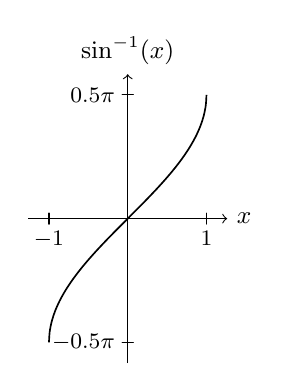
\begin{tikzpicture}
\datavisualization[school book axes, visualize as smooth line, y axis={ticks={step=(pi/2), major={at={(-pi/2),(pi/2)}}, tick typesetter/.code=\mytypesetter{##1}}, label=$\sin^{-1}(x)$}, x axis={label=$x$}]
data[format=function]{
	var y : interval [-pi/2:pi/2];
	func x = sin(\value{y} r);
};
\end{tikzpicture}\\[1ex]
\end{center}
(3)$\cos^{-1}$既不是偶函数也不是奇函数; 其定义域为$[-1,1]$, 值域为$[0,\pi]$.\\[1ex]
(4)$\displaystyle\frac{d}{dx}\cos^{-1}(x)=-\frac{1}{\sqrt{1-x^2}}$, 其中$-1<x<1$.\\[1ex]
\begin{center}
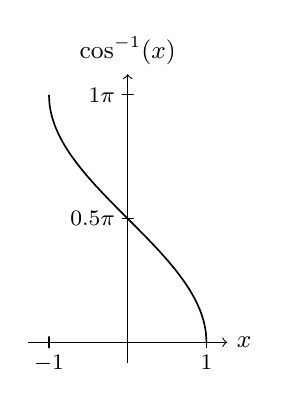
\begin{tikzpicture}
\datavisualization[school book axes, visualize as smooth line, y axis={ticks={step=(pi/2), major={at={(pi/2),(pi)}}, tick typesetter/.code=\mytypesetter{##1}}, label=$\cos^{-1}(x)$}, x axis={label=$x$}]
data[format=function]{
	var y : interval [0:pi];
	func x = cos(\value{y} r);
};
\end{tikzpicture}\\[1ex]
\end{center}
(5)$\tan^{-1}$是奇函数; 其定义域是$\mathbb{R}$且值域是$\displaystyle(-\frac{\pi}{2},\frac{\pi}{2})$.\\[1ex]
(6)对于所有的实数$x$, $\displaystyle\frac{d}{dx}\tan^{-1}(x)=\frac{1}{1+x^2}$.\\[1ex]
\begin{center}
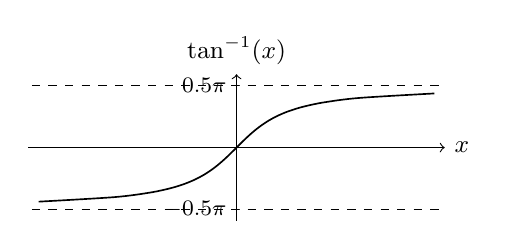
\begin{tikzpicture}[scale=0.5]
\datavisualization[school book axes, visualize as smooth line, y axis={ticks={step=(pi/2), major={at={(-pi/2),(pi/2)}}, tick typesetter/.code=\mytypesetter{##1}}, include value={-1.6,1.6}, label=$\tan^{-1}(x)$}, x axis={ticks=none, label=$x$}]
data[format=function]{
    var y : interval [-pi*7/16:pi*7/16];
    func x = tan(\value{y} r);
};
\draw[dashed] (-5.2, pi/2) -- (5.2, pi/2);
\draw[dashed] (-5.2, -pi/2) -- (5.2, -pi/2);
\end{tikzpicture}\\[1ex]
\end{center}
(7)$\cot^{-1}$既不是奇函数也不是偶函数; 其定义域为$\mathbb{R}$且值域是$(0,\pi)$\\[1ex]
(8)对于所有的实数$x$, $\displaystyle\frac{d}{dx}\cot^{-1}(x)=-\frac{1}{1+x^2}$.\\[1ex]
\begin{center}
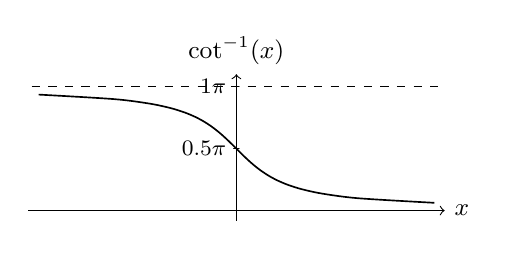
\begin{tikzpicture}[scale=0.5]
\datavisualization[school book axes, visualize as smooth line, y axis={ticks={step=(pi/2), major={at={(pi/2),(pi)}}, tick typesetter/.code=\mytypesetter{##1}}, include value={3.2}, label=$\cot^{-1}(x)$}, x axis={ticks=none, label=$x$}]
data[format=function]{
    var y : interval [pi*1/16:pi*15/16];
    func x = cot(\value{y} r);
};
\draw[dashed] (-5.2, pi) -- (5.2, pi);
\end{tikzpicture}
\end{center}
(9)$\sec^{-1}$既不是奇函数也不是偶函数; 其定义域是$(-\infty,-1]\cup[1,\infty)$且值域是$\displaystyle[0,\frac{\pi}{2})\cup(\frac{\pi}{2},\pi]$.\\[1ex]
(10)对于$x>1$或$x<-1$, $\displaystyle\frac{d}{dx}\sec^{-1}(x)=\frac{1}{|x|\sqrt{x^2-1}}$.\\[1ex]
\begin{center}
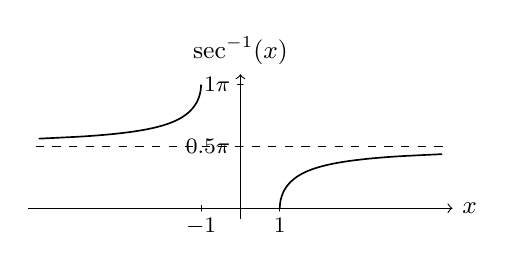
\begin{tikzpicture}[scale=0.5]
\datavisualization[school book axes, visualize as smooth line/.list={sec1, sec2}, y axis={ticks={step=(pi/2), major={at={(pi/2),(pi)}}, tick typesetter/.code=\mytypesetter{##1}}, label=$\sec^{-1}(x)$}, x axis={ticks={major={at={-1,0,1}}}, label=$x$}]
data [set=sec1, format=function] {
var y : interval [0:pi*7/16];
func x = 1/cos(\value y r);
}
data [set=sec2,format=function] {
var y : interval [pi*9/16:pi];
func x = 1/cos(\value y r);
};
\draw[dashed] (-5.2, 0.5*pi) -- (5.2, 0.5*pi);
\end{tikzpicture}
\end{center}
(11)$\csc^{-1}$是奇函数; 其定义域为$(-\infty,-1]\cup[1,\infty)$且值域是$\displaystyle[-\frac{\pi}{2},0)\cup(0,\frac{\pi}{2}]$.\\[1ex]
(12)对于$x>1$或$x<-1$, $\displaystyle\frac{d}{dx}\csc^{-1}(x)=-\frac{1}{|x|\sqrt{x^2-1}}$.\\[2ex]
\begin{center}
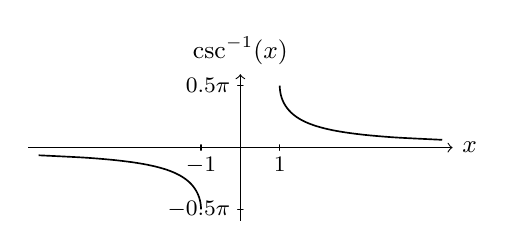
\begin{tikzpicture}[scale=0.5]
\datavisualization[school book axes, visualize as smooth line/.list={csc1, csc2}, y axis={ticks={step=(pi/2), major={at={(-pi/2),(pi/2)}}, tick typesetter/.code=\mytypesetter{##1}}, include value={-1.6,1.6}, label=$\csc^{-1}(x)$}, x axis={ticks={major={at={-1,0,1}}}, label=$x$}]
data [set=csc1, format=function] {
var y : interval [pi*1/16:pi/2];
func x = 1/sin(\value y r);
}
data [set=csc2,format=function] {
var y : interval [-pi/2:-pi*1/16];
func x = 1/sin(\value y r);
};
\end{tikzpicture}
\end{center}\vspace{2ex}

4.计算反三角函数\\
化简形如$\sin^{-1}(\sin(\alpha))$的三角函数:\\
\phantom{(1)}获取指定角$\alpha$的参照角\\
\phantom{(1)}找到反三角函数定义域中拥有该参照角的角\\
\phantom{(1)}确定该角的正弦值与$\alpha$参照角的正弦值符号一致\\[2ex]

5.反双曲函数\\
(1)$\sinh^{-1}$是奇函数; 其定义域和值域都是$\mathbb{R}$.\\[1ex]
(2)对于所有的实数$x$, $\displaystyle\frac{d}{dx}\sinh^{-1}(x)=\frac{1}{\sqrt{x^2+1}}$.\\[1ex]
(3)$\cosh^{-1}$既不是奇函数也不是偶函数; 其定义域是$[1,\infty)$且值域是$[0,\infty)$.\\[1ex]
(4)对于$x>1$, $\displaystyle\frac{d}{dx}\cosh^{-1}(x)=\frac{1}{\sqrt{x^2-1}}$.\\[1ex]
\end{document}

\chapter{导数和图像}
1.函数的极值
\begin{theorem}[极值定理]
假设函数$f$定义在开区间$(a,b)$内, 并且点$c$在$(a,b)$区间内. 如果点$c$为函数的局部最大值或最小值, 那么点$c$一定为该函数的临界点. 也就是说, $f'(c)=0$或$f'(c)$不存在.
\end{theorem}
求解闭区间$[a,b]$内的全局最大值和最小值步骤:\\
(1)求出$f'(x)$, 并列出在$(a,b)$中$f'(x)$不存在或$f'(x)=0$的点. 也就是说, 列出在开区间$(a,b)$内所有的临界点.\\
(2)把端点$x=a$和$x=b$放入列表.\\
(3)对于上述列表中的每个点, 将它们带入$y=f(x)$求出对应函数值.\\
(4)找出最大的函数值以及它所对应的$x$值, 得到全局最大值.\\
(5)类似于(4), 得到全局最小值.\\[2ex]

2.罗尔定理
\begin{theorem}[罗尔定理]
假设函数$f$在闭区间$[a,b]$内连续, 在开区间$(a,b)$内可导. 如果$f(a)=f(b)$, 那么在开区间$(a,b)$内至少存在一点$c$, 使得$f'(c)=0$.
\end{theorem}\vspace{4ex}

3.中值定理
\begin{theorem}[中值定理]
假设函数$f$在闭区间$[a,b]$内连续, 在开区间$(a,b)$内可导, 那么在开区间$(a,b)$内至少有一点$c$使得
\[f'(x)=\frac{f(b)-f(a)}{b-a}\]
\end{theorem}
\framebox{
\begin{minipage}{\linewidth}
如果对于在定义域$(a,b)$内的所有$x$, 都有$f'(x)=0$, 那么函数$f$在开区间$(a,b)$内为常数函数.
\end{minipage}}\\[2ex]
\framebox{
\begin{minipage}{\linewidth}
如果对于任意实数$x$都有$f'(x)=g'(x)$, 那么有$f(x)=g(x)+C$($C$为常数).
\end{minipage}}\\[4ex]

4.二阶导数与图像
{\par\raggedright
\framebox{如果$x=c$点是函数$f$的拐点, 则有$f''(c)=0$.}\\[2ex]
\framebox{如果$f''(c)=0$, 则$c$点不一定都是函数$f$的拐点.}\par}\vspace{4ex}

5.导数为零的汇总\\
纯1阶导数分析 - 假设$f'(c)=0$, 此时情况如下:\\
(1)如果从左往右通过$c$点, $f'(x)$的符号由正变负, 那么$c$点为局部最大值;\\
(2)如果从左往右通过$c$点, $f'(x)$的符号由负变正, 那么$c$点为局部最小值;\\
(3)如果从左往右通过$c$点, $f'(x)$的符号不发生变化, 那么$c$点为水平拐点.

1/2阶导数综合分析 - 假设$f'(x)=0$, 则有:\\
(1)如果$f''(c)<0$, 那么$x=c$为局部最大值;\\
(1)如果$f''(c)>0$, 那么$x=c$为局部最小值;\\
(1)如果$f''(c)=0$, 那么无法判断, 需借助纯1阶分析\\

\documentclass[UTF8, fontset=ubuntu]{ctexart}
\usepackage{parskip}
\begin{document}
1.建立原函数的符号表格\\
(1)建立一个两行的表格, 第一行为$x$取值, 第二行为$f(x)$对应值;\\
(2)在第一行以递增顺序列出$x$所有的关于$f(x)$的零点和不连续点, 并且每个数的左右都要留出表格;\\
(3)填充第二行, 零点直接填0, 不连续点以'*'填充;\\
(4)在第一行第一个数左边填上小于该数的数字, 在中间两个数之间填上介于之间的数字, 在最后一个数字右边填上大于该数的数字;\\
(5)根据第(4)步的值, 在第二行计算对应$f(x)$的值, 大于0则填上'+', 小于0则填上'-'.\\[2ex]

2.建立一阶导数的符号表格\\
(1)建立一个三行行的表格, 第一行为$x$取值, 第二行为$f'(x)$对应值, 第三行为趋势图;\\
(2)在第一行以递增顺序列出$x$所有的关于$f'(x)$的零点和不连续点, 并且每个数的左右都要留出表格;\\
(3)填充第二行, 零点直接填0, 不连续点以'*'填充;\\
(4)在第一行第一个数左边填上小于该数的数字, 在中间两个数之间填上介于之间的数字, 在最后一个数字右边填上大于该数的数字;\\
(5)根据第(4)步的值, 在第二行计算对应$f'(x)$的值, 大于0则填上'+', 小于0则填上'-';\\
(6)在第三行根据第二行的内容, 在该列填上对应内容, '+'对应'/', '0'对应'—', '-'对应'\'.\\[2ex]

3.建立二阶导数的符号表格\\
(1)建立一个两行的表格, 第一行为$x$取值, 第二行为$f''(x)$对应值, 第三行为趋势图;\\
(2)在第一行以递增顺序列出$x$所有的关于$f''(x)$的零点和不连续点, 并且每个数的左右都要留出表格;\\
(3)填充第二行, 零点直接填0, 不连续点以'*'填充;\\
(4)在第一行第一个数左边填上小于该数的数字, 在中间两个数之间填上介于之间的数字, 在最后一个数字右边填上大于该数的数字;\\
(5)根据第(4)步的值, 在第二行计算对应$f'(x)$的值, 大于0则填上'+', 小于0则填上'-';\\
(6)在第三行根据第二行的内容, 在该列填上对应内容, '+'对应'∪'', '0'对应'.', '-'对应'∩'.\\[2ex]

4.绘制函数图像的完整步骤\\
(1)对称性 - 通过$-x$替换$x$, 来验证函数的奇偶性;\\
(2)$y$轴截距 - 通过$x=0$来求$y$轴截距;\\
(3)$x$轴截距 - 通过$y=0$来求$x$轴截距;\\
(4)定义域 - 除已直接给出定义域的情况, 可剔除使得分母为0、偶数根号下的量为负数、对数符号里的量为负数或0的数, 并且反三角函数也需注意;\\
(5)垂直渐近线 - 分母为0且分子不为0的位置, 或对数式;\\
(6)函数的正负 - 建立关于$f(x)$的符号表格;\\
(7)水平渐近线 - 通过计算$\lim_{x\to\infty}f(x)$和$\lim_{x\to -\infty}f(x)$来找出函数的水平渐近线;
(8)导数的正负 - 绘制关于一阶导数的符号表格;\\
(9)最大值和最小值 - 根据(8)的符号表格, 计算所有局部最大/小值, 找出全局最大/小值;\\
(10)二阶导数的正负 - 绘制关于二阶导数的符号表格;\\
(11)拐点 - 拐点的二阶导数为0, 并且在该点两侧导数的正反符号相反.\\[2ex]
\end{document}

\documentclass[UTF8, fontset=ubuntu]{ctexart}
\usepackage{parskip}
\begin{document}

\end{document}

\chapter{洛必达法则及极限问题总结}
1.类型$A$: $\displaystyle\frac{0}{0}$
{\par\raggedright
\framebox{如果$f(a)=g(a)=0$, 那么$\displaystyle\lim_{x\to a}\frac{f(a)}{g(a)}=\lim_{x\to a}\frac{f'(x)}{g'(x)}$}\
\par}\vspace{2ex}
例.\\
\phantom{例}$\displaystyle\lim_{x\to 0}\frac{x-\sin x}{x^3}$\\
$\displaystyle\lim_{x\to 0}\frac{x-\sin x}{x^3}=\lim_{x\to 0}\frac{1-\cos x}{3x^2}=\lim_{x\to 0}\frac{\sin x}{6x}=\frac{1}{6}$\\[2ex]

2.类型$A$: $\displaystyle\frac{\pm\infty}{\pm\infty}$
{\par\raggedright
\framebox{如果$f(a)=g(a)=\pm\infty$, 那么$\displaystyle\lim_{x\to a}\frac{f(a)}{g(a)}=\lim_{x\to a}\frac{f'(x)}{g'(x)}$}
\par}\vspace{2ex}
例1.\\
\phantom{例}$\displaystyle\lim_{x\to\infty}\frac{3x^2+7x}{2x^2-5}$\\
$\displaystyle\lim_{x\to\infty}\frac{3x^2+7x}{2x^2-5}=\lim_{x\to\infty}\frac{6x+7}{4x}=\lim_{x\to\infty}(\frac{6}{4}+\frac{7}{4x})=\frac{3}{2}$\\[2ex]

例2.\\
\phantom{例}$\displaystyle\lim_{x\to 0^+}\frac{\csc x}{1-\ln x}$\\
$\displaystyle\lim_{x\to 0^+}\frac{\csc x}{1-\ln x}=\lim_{x\to 0^+}\frac{-\csc x\cot x}{-\frac{1}{x}}=\lim_{x\to 0^+}\frac{x}{\sin x}\frac{1}{\tan x}=1\times\infty=\infty$\\[2ex]

例3.\\
\phantom{例}$\displaystyle\lim_{x\to\infty}\frac{x}{e^x}$\\
$\displaystyle\lim_{x\to\infty}\frac{x}{e^x}=\lim_{x\to\infty}\frac{1}{e^x}=0$\\[2ex]

3.类型$B1$: $\infty -\infty$\\
方法: 通过通分或者分子/分母同时乘以共轭表达式来转化为类型$A$\\
例.\\
\phantom{例}$\displaystyle\lim_{x\to 0}(\frac{1}{\sin x}-\frac{1}{x})$\\
$\displaystyle\lim_{x\to 0}(\frac{1}{\sin x}-\frac{1}{x})=\lim_{x\to 0}\frac{x-\sin x}{x\sin x}=\lim_{x\to 0}\frac{1-\cos x}{\sin x+x\cos x}$\\
$\displaystyle\phantom{\lim_{x\to 0}(\frac{1}{\sin x}-\frac{1}{x})}=\lim_{x\to 0}\frac{\sin x}{2\cos x-x\sin x}=0$\\[2ex]

4.类型$B2$: $0\times\pm\infty$\\
方法: 选择两个因式中较简单的那个取倒数把它移到分母(尽量不要选用对数做分母, 把它留在分子)\\
例.\\
\phantom{例}$\displaystyle\lim_{x\to 0^+}x\ln x$\\
$\displaystyle\lim_{x\to 0^+}x\ln x=\lim_{x\to 0^+}\frac{\ln x}{\frac{1}{x}}=\lim_{x\to 0^+}\frac{\frac{1}{x}}{-\frac{1}{x^2}}=\lim_{x\to 0^+}(-x)=0$\\[2ex]

5.类型$C$: $1^{\pm\infty}$,$0^0$,$\infty^0$\\
通过取对数, 转化为类型$B2$或$A$, 计算获得极限$L$, 再以$e$为底/$L$为幂获取最终结果\\
例1.\\
\phantom{例}$\displaystyle\lim_{x\to 0^+}x^{\sin x}$\\
$\displaystyle\lim_{x\to 0^+}\ln(x^{\sin x})=\lim_{x\to 0^+}\sin x\ln x=\lim_{x\to 0^+}\frac{\ln x}{\csc x}=\lim_{x\to 0^+}\frac{\frac{1}{x}}{-\csc x\cot x}$\\
$\displaystyle\phantom{\lim_{x\to 0^+}\ln(x^{\sin x})}=\lim_{x\to 0^+}-\frac{\sin x}{x}\times\tan x=0$\\
对两边求指数, 得:\\
$\displaystyle\lim_{x\to 0^+}x^{\sin x}=e^0=1$\\[2ex]

例2.\\
\phantom{例}$\displaystyle\lim_{x\to 0}(1+3\tan x)^{\frac{1}{x}}$\\
$\displaystyle\lim_{x\to 0}\ln((1+3\tan x)^{\frac{1}{x}})=\lim_{x\to 0}\frac{\ln(1+3\tan x)}{x}=\lim_{x\to 0}\frac{\frac{3\sec^2x}{1+3\tan x}}{1}$\\
$\displaystyle\phantom{\lim_{x\to 0}\ln((1+3\tan x)^{\frac{1}{x}})}=\frac{3\times1^2}{1+3\times0}=3$\\
对两边求指数, 得:\\
$\displaystyle\lim_{x\to 0}(1+3\tan x)^{\frac{1}{x}}=e^3$

%最后编辑于: 2021-12-28

\documentclass[UTF8, fontset=ubuntu]{ctexart}
\usepackage{parskip}
\usepackage{amsmath}
\begin{document}
如下公式:\\
\[\sum_{j=1}^n\frac{1}{j^2}\]
代表从$j=1$到$j=n$时, $\displaystyle\frac{1}{j^2}$的和.\\
n为唯一\textbf{变量}.\\
j为\textbf{虚拟变量}, 也称为\textbf{求和指标}.\\[2ex]

常用求和公式:
\begin{gather}
\sum_{j=1}^n j=\frac{n(n+1)}{2}\\
\sum_{j=1}^b j^2=\frac{n(n+1)(2n+1)}{6}
\end{gather}
\end{document}

\chapter{定积分}
1.公式
\[\int_a^bf(x)dx\]
为\textbf{定积分}, 表示``函数$f(x)$对于$x$从$a$到$b$的积分''.\\
$f(x)$为\textbf{被积函数}.\\
$a$和$b$为\textbf{积分极限}, 也称为\textbf{积分端点}.\\

2.有向面积积分:\\[1ex]
\framebox{
\begin{minipage}{\linewidth}
$\int_a^bf(x)dx$是由曲线$y=f(x)$, 两条垂线$x=a$和$x=b$, 以及$x$轴所围成的有向面积(平方单位).
\end{minipage}}\vspace{4ex}

3.定积分公式:\\
\begin{center}
\framebox{$\displaystyle\int_b^af(x)dx=-\int_a^bf(x)dx$.}\\[2ex]
\framebox{$\displaystyle\int_a^af(x)dx=0$.}\\[2ex]
\framebox{$\displaystyle\int_a^bf(x)dx=\int_a^cf(x)dx+\int_c^bf(x)dx$.}\\[2ex]
\framebox{$\displaystyle\int_a^bCf(x)dx=C\int_a^bf(x)dx$.}\\[2ex]
\framebox{$\displaystyle\int_a^b(f(x)+g(x))dx=\int_a^bf(x)dx+\int_a^bg(x)dx$.}\\
\end{center}\vspace{4ex}

4.两条曲线之间的面积:\\[1ex]
\framebox{在函数$f$和$g$之间的面积(平方单位)$\displaystyle =\int_a^b|f(x)-g(x)|dx$.}\\[2ex]

5.曲线与$y$轴围成的面积:\\[1ex]
\framebox{
\begin{minipage}{\linewidth}
如果$f$存在反函数, $\displaystyle\int_A^Bf^{-1}(y)dy$就是由函数$y=f(x)$、直线$y=A$和$y=B$以及$y$轴所围成的面积(平方单位).
\end{minipage}}\vspace{4ex}

6.积分比较:\\[1ex]
\framebox{
\begin{minipage}{\linewidth}
如果对于在区间$[a,b]$内的所有$x$都有$f(x)\leqslant g(x)$, 那么就有
\[\int_a^bf(x)dx\leqslant\int_a^bg(x)dx.\]
\end{minipage}}\vspace{4ex}

7.简单估算:\\[1ex]
\framebox{
\begin{minipage}{\linewidth}
如果对于在$[a,b]$区间内的所有$x$有$m\leqslant f(x)\leqslant M$, 那么
\[m(b-a)\leqslant\int_a^bf(x)dx\leqslant M(b-a).\]
\end{minipage}}\vspace{4ex}

8.积分的平均值:\\[1ex]
\framebox{函数$f$在区间$[a,b]$内的平均值$\displaystyle=\frac{1}{b-a}\int_a^bf(x)dx$.}\vspace{4ex}

9.积分的中值定理:\\[1ex]
\framebox{
\begin{minipage}{\linewidth}
如果函数$f$在闭区间$[a,b]$上连续, 那么在开区间$(a,b)$内总有一点$c$, 满足$\displaystyle f(c)=\frac{1}{b-a}\int_a^bf(x)dx$.
\end{minipage}}

\chapter{微积分的基本定理}
1.第一基本定理\\[-4ex]
\begin{theorem}[微积分的第一基本定理:]
如果函数$f$在闭区间$[a,b]$上是连续的, 定义$F$为
\[F(x)=\int_a^xf(t)\dif t,\ x\in[a,b]\]
则$F$在开区间$(a,b)$内是可导函数, 而且$F'(x)=f(x)$.
\end{theorem}\vspace{4ex}

2.第二基本定理\\[-4ex]
\begin{theorem}[微积分的第二基本定理:]
如果函数$f$在闭区间$[a,b]$上是连续的, $F$是$f$的任意一个反导数$(\text{关于}x)$, 那么有
\[\int_a^bf(x)\dif x=F(b)-F(a)=F(x)\Big|_a^b\]
\end{theorem}\vspace{4ex}

3.不定积分法则\\[1ex]
\framebox{如果$\displaystyle\frac{\dif}{\dif x}F(x)=f(x)$, 那么$\displaystyle\int f(x)\dif x=F(x)+C$.}\\[4ex]

4.不定积分运算法则\\[-4ex]
\begin{center}
\framebox{$\displaystyle\int (f(x)+g(x))dx=\int f(x)\dif x+\int g(x)\dif x$}\\[2ex]
\framebox{$\displaystyle\int Cf(x)\dif x=C\int f(x)\dif x$}
\end{center}\vspace{4ex}

5.微分和积分对照公式\\
\begin{displaymath}
\begin{array}{l l}
\dfrac{\dif}{\dif x}x^a=ax^{a-1} & \displaystyle\int x^a\dif x=\dfrac{x^{a+1}}{a+1}+C(a\neq -1)\\[2ex]
\dfrac{\dif}{\dif x}\ln(x)=\dfrac{1}{x} & \displaystyle\int\dfrac{1}{x}\dif x=\ln|x|+C\\[2ex]
\dfrac{\dif}{\dif x}e^x=e^x & \displaystyle\int e^x\dif x=e^x+C\\[2ex]
\dfrac{\dif}{\dif x}b^x=b^x\ln(b) & \displaystyle\int b^x\dif x=\dfrac{b^x}{\ln(b)}+C\\[2ex]
\dfrac{\dif}{\dif x}\sin(x)=\cos(x) & \displaystyle\int \cos(x)\dif x=\sin(x)+C\\[2ex]
\dfrac{\dif}{\dif x}\cos(x)=-\sin(x) & \displaystyle\int \sin(x)\dif x=-\cos(x)+C\\[2ex]
\dfrac{\dif}{\dif x}\tan(x)=\sec^2(x) & \displaystyle\int \sec^2(x)\dif x=\tan(x)+C\\[2ex]
\dfrac{\dif}{\dif x}\sec(x)=\sec(x)\tan(x) & \displaystyle\int \sec(x)\tan(x)\dif x=\sec(x)+C\\[2ex]
\dfrac{\dif}{\dif x}\cot(x)=-\csc^2(x) & \displaystyle\int \csc^2(x)\dif x=-\cot(x)+C\\[2ex]
\dfrac{\dif}{\dif x}\csc(x)=-\csc(x)\cot(x) & \displaystyle\int \csc(x)\cot(x)\dif x=-\csc(x)+C\\[2ex]
\dfrac{\dif}{\dif x}\sin^{-1}(x)=\dfrac{1}{\sqrt{1-x^2}} & \displaystyle\int \dfrac{1}{\sqrt{1-x^2}}\dif x=\sin^{-1}(x)+C\\[2ex]
\dfrac{\dif}{\dif x}\tan^{-1}(x)=\dfrac{1}{1+x^2} & \displaystyle\int \dfrac{1}{1+x^2}\dif x=\tan^{-1}(x)+C\\[2ex]
\dfrac{\dif}{\dif x}\sec^{-1}(x)=\dfrac{1}{|x|\sqrt{x^2-1}} & \displaystyle\int \dfrac{1}{|x|\sqrt{x^2-1}}\dif x=\sec^{-1}(x)+C\\[2ex]
\dfrac{\dif}{\dif x}\sinh(x)=\cosh(x) & \displaystyle\int \cosh(x)\dif x=\sinh(x)+C\\[2ex]
\dfrac{\dif}{\dif x}\cosh(x)=\sinh(x) & \displaystyle\int \sinh(x)\dif x=\cosh(x)+C
\end{array}
\end{displaymath}

\chapter{积分的方法 I}
1.换元法
{\par\centering
\framebox{$\displaystyle\int\frac{f'(x)}{f(x)}\dif x=\ln|f(x)|+C$.}
\par}
例.\\[1ex]
$\displaystyle\int\frac{x}{x^2+8}\dif x$\\[1ex]
推导过程:\\[1ex]
$\displaystyle\because\frac{\dif}{\dif x}(x^2+8)=2x$\\[1ex]
$\therefore$使用换元法, 设$t=x^2+8$.\\[1ex]
\phantom{$\therefore$}得到$\dif t=2x\dif x$\\[1ex]
$\therefore\displaystyle\int\frac{x}{x^2+8}\dif x=\frac{1}{2}\int\frac{1}{t}\dif t=\frac{1}{2}\ln|t|+C=\frac{1}{2}\ln|x^2+8|+C$\\[2ex]

2.形如$\sqrt[b]{ax+b}$的积分
{\par\centering
\framebox{在换掉$\sqrt[n]{ax+b}$之前, 设$t=\sqrt[n]{ax+b}$并对等式$t^n=ax+b$两端求导.}
\par}
例.\\[1ex]
$\displaystyle\int x\sqrt[5]{3x+2}\dif x$\\[1ex]
推导过程:\\[1ex]
设$t=\sqrt[5]{3x+2}$, 得:\\[1ex]
$\displaystyle x=\frac{1}{3}(t^5-2)$\\[1ex]
等式两端$5$次方并求导, 得:\\[1ex]
$\displaystyle\dif x=\frac{5}{3}t^4\dif t$\\[1ex]
$\displaystyle\therefore\int x\sqrt[5]{3x+2}\dif x=\frac{5}{9}\int(t^{10}-2t^5)\dif t=\frac{5}{9}\int t^{10}\dif t-\frac{10}{9}\int t^5\dif t$\\[1ex]
$\displaystyle\phantom{\therefore\int x\sqrt[5]{3x+2}\dif x}=\frac{5}{99}t^{11}-\frac{5}{27}t^6+C$\\[1ex]
将$t=\sqrt[5]{3x+2}$代入上述等式, 得:\\[1ex]
$\displaystyle\int x\sqrt[5]{3x+2}\dif x=\frac{5}{99}(3x+2)^{\frac{11}{5}}-\frac{5}{27}(3x+2)^{\frac{6}{5}}+C$\\[2ex]

3.分部积分法
{\par\centering
\framebox{$\displaystyle\int u\frac{\dif v}{\dif x}\dif x=uv-\int v\frac{\dif u}{\dif x}\dif x$.}
\par}
例.\\[1ex]
$\displaystyle\int xe^x\dif x$\\[1ex]
推导过程:\\[1ex]
设$u=x$, $v=e^x$, 得:\\[1ex]
$\displaystyle\int xe^x\dif x=xe^x-\int e^x\dif x$\\[1ex]
$\displaystyle\int xe^x\dif x=xe^x-e^x+C$\\[2ex]

4.部分分式
{\par\centering
\framebox{
\begin{minipage}{\linewidth}
部分分式处理步骤:\\
(1)查看分子分母最高项的次数, 如有必要(分子次数$\geqslant$分母次数)做除法;\\
(2)对分母进行因式分解;\\
(3)进行"分部", 分部类别如下:\\[1ex]
	\phantom{\qquad}1)\,线性式:$\displaystyle\frac{A}{x+a}$\\[1ex]
	\phantom{\qquad}2)\,线性式的平方:$\displaystyle\frac{A}{(x+a)^2}+\frac{B}{x+a}$\\[1ex]
	\phantom{\qquad}3)\,二次多项式:$\displaystyle\frac{Ax+B}{x^2+ax+b}$\\[1ex]
	\phantom{\qquad}4)\,线性式的三次方:$\displaystyle\frac{A}{(x+a)^3}+\frac{B}{(x+a)^2}+\frac{C}{x+a}$\\[1ex]
	\phantom{\qquad}5)\,线性式的四次方:$\displaystyle\frac{A}{(x+a)^4}+\frac{B}{(x+a)^3}+\frac{C}{(x+a)^2}+\frac{D}{x+a}$\\
(4)计算分部中分子常数的值;\\
(5)求解分母为线性项次幂的积分, 即(3)中的1)/2)/4)/5)类型. 涉及到对数或负次幂;\\
(6)求解分母为二次多项式的积分, 即(3)中的3)类型. 具体方法: 先配方, 再换元. 涉及到对数和正切函数.
\end{minipage}}
\par}
例.\\[1ex]
$\displaystyle\int\frac{x+2}{x^2-1}\dif x$\\[1ex]
推导过程:\\[1ex]
对分母$x^2-1$进行因式分解:\\[1ex]
$x^2-1=(x+1)(x-1)$\\[1ex]
进行分部:\\[1ex]
$\displaystyle\frac{x+2}{x^2-1}=\frac{A}{x+1}+\frac{B}{x-1}$\\[1ex]
求分子常数的值:\\[1ex]
$\displaystyle A(x-1)+B(x+1)=x+2\quad\Rightarrow\quad\left\{
\begin{array}{l}
A+B=1\\
B-A=2
\end{array}\right.\quad\Rightarrow\quad A=-\frac{1}{2},B=\frac{3}{2}$\\[1ex]
求解分母为线性次幂的积分:\\[1ex]
$\displaystyle\int\frac{x+2}{x^2-1}\dif x=\frac{3}{2}\int\frac{1}{x-1}\dif x-\frac{1}{2}\int\frac{1}{x+1}\dif x=\frac{3}{2}\ln|x-1|-\frac{1}{2}\ln|x+1|+C$

\chapter{积分的方法 II}
1.三角恒等式\\
(1)形如$\sqrt{1\pm\cos(x)}$\\
例.\\
$\displaystyle\int_0^{\frac{\pi}{2}}\sqrt{1-\cos(2x)}\dif x$\\
推导原理:\\
将一个数与三角函数的运算, 转化为该三角函数半角的三角函数平方, 便于开根号\\
推导过程:\\
由$\cos(2x)=1-2\sin^2(x)$, 得:\\
$\displaystyle\int_0^{\frac{\pi}{2}}\sqrt{1-\cos(2x)}\dif x=\sqrt{2}\int_0^{\frac{\pi}{2}}|\sin(x)|\dif x$\\
由于$\sin(x)$在定义域区间$[0,\frac{\pi}{2}]$内为正, 所以:\\
$\displaystyle\int_0^{\frac{\pi}{2}}\sqrt{1-\cos(2x)}\dif x=-\sqrt{2}\cos(x)\Big{|}_0^{\frac{\pi}{2}}=0-(-\sqrt{2})=\sqrt{2}$\\

(2)形如$\sqrt{1-\sin^2(x)}/\sqrt{1+\tan^2(x)}$\\
例.\\
$\displaystyle\int_0^{\pi}\sqrt{1-\cos^2(x)}\dif x$\\
推导原理:\\
将根号下一个数字与三角函数平方的运算, 转化为该三角函数角的另一个三角函数的平方, 便于开根号\\
推导过程:\\
由$\sin^2(x)=1-\cos^2(x)$, 得:\\
$\displaystyle\int_0^{\pi}\sqrt{1-\cos^2(x)}\dif x=\int_0^{\pi}\sqrt{sin^2(x)}\dif x=\int_0^{\pi}|\sin(x)|\dif x$\\
由于$\sin(x)$在区间$[0,\pi]$内为正, 所以:\\
$\displaystyle\int_0^{\pi}\sqrt{1-\cos^2(x)}\dif x=\int_0^{\pi}\sin(x)\dif x=-\cos(x)\Big{|}_0^{\pi}=1-(-1)=2$\\

(3)形如$\displaystyle\frac{1}{\sec(x)-1}$\\
例.\\
$\displaystyle\int\frac{1}{\sec(x)-1}\dif x$\\
推导原理:\\
将分子分母同时乘以分母的共轭式\\
推导过程:\\
$\displaystyle\int\frac{1}{\sec(x)-1}\dif x=\int\frac{1}{\sec(x)-1}\times\frac{\sec(x)+1}{\sec(x)+1}\dif x=\int\frac{\sec(x)+1}{\sec^2(x)-1}\dif x$\\
\phantom{$\displaystyle\int\frac{1}{\sec(x)-1}\dif x$}$\displaystyle=\int\frac{\sec(x)}{\tan^2(x)}\dif x+\int\frac{1}{\tan^2(x)}\dif x=\int\frac{\cos(x)}{\sin^2(x)}\dif x+\int\frac{1}{\tan^2(x)}\dif x$\\
设$t=\sin(x)$, 则$\dif t=\cos(x)\dif x$, 得:\\
$\displaystyle\int\frac{\cos(x)}{\sin^2(x)}\dif x=\int\frac{1}{t^2}\dif t=-\frac{1}{t}+C=-\csc(x)+C$\\
由$\displaystyle\frac{\dif}{\dif x}\cot(x)=-\csc^2(x)$, 得:\\
$\displaystyle\int\frac{1}{\tan^2(x)}\dif x=\int\cot^2(x)\dif x=\int\csc^2(x)\dif x-\int\dif x=-\cot(x)-x+C$\\
$\therefore\displaystyle\int\frac{1}{\sec(x)-1}\dif x=-\csc(x)-\cot(x)-x+C$\\

(4)形如$\sin(\alpha)\cos(\beta)$\\
例.\\
$\displaystyle\int\sin(19x)\cos(3x)\dif x$\\
推导原理:\\
利用和/差角公式:\\[-4ex]
\begin{center}
    \framebox{$\sin(A+B)=\sin(A)\cos(B)+\cos(A)\sin(B)$}\\[2ex]
    \framebox{$\cos(A+B)=\cos(A)\cos(B)-\sin(A)\sin(B)$}\\[2ex]
    \framebox{$\sin(A-B)=\sin(A)\cos(B)-\cos(A)\sin(B)$}\\[2ex]
    \framebox{$\cos(A-B)=\cos(A)\cos(B)+\sin(A)\sin(B)$}
\end{center}\vspace{1ex}
可推断出:\\[-4ex]
\begin{center}
	\framebox{$\sin(A)\cos(B)=\dfrac{1}{2}(\sin(A+B)+\sin(A-B))$}\\[2ex]
	\framebox{$\cos(A)\cos(B)=\dfrac{1}{2}(\cos(A+B)+\cos(A-B))$}\\[2ex]
	\framebox{$\sin(A)\sin(B)=\dfrac{1}{2}(\cos(A-B)-\cos(A+B))$}\\[2ex]
\end{center}\newpage
推导过程:\\
$\displaystyle\therefore\int\sin(19x)\cos(3x)\dif x=\frac{1}{2}\int(\sin(19x+3x)+\sin(19x-3x))\dif x$\\
$\displaystyle\phantom{\therefore\int\sin(19x)\cos(3x)\dif x}=\frac{1}{2}\int(\sin(22x)+\sin(16x))\dif x$\\
$\displaystyle\phantom{\therefore\int\sin(19x)\cos(3x)\dif x}=\frac{1}{2}\left(-\frac{\cos(22x)}{22}-\frac{\cos(16x)}{16}\right)+C$\\
$\displaystyle\phantom{\therefore\int\sin(19x)\cos(3x)\dif x}=-\frac{\cos(22x)}{44}-\frac{\cos(16x)}{32}+C$\\[4ex]

2.关于三角函数的幂的积分\\
(1)$\sin$或$\cos$的幂\\
I、至少一个乘积项为奇次幂\\
例.\\
$\displaystyle\int\sin^7(x)\cos^4(x)\dif x$\\
解题思路:\\
将奇次幂分解为1次方和n-1次方, 并且将剩下的n-1偶次幂利用$\cos^2(x)+\sin^2(x)=1$进行转化\\
推导过程:\\
设$t=\cos(x)$, 则$\dif t=-\sin(x)\dif x$, 得:\\
\(\begin{array}{>{\displaystyle}r >{\displaystyle}l}
\int\sin^7(x)\cos^4(x)\dif x & =-\int\sin^6(x)\cos^4(x)(-\sin(x)\dif x)\\
& =-\int(1-\cos^2(x))^3\cos^4(x)(-\sin(x)\dif x)\\
& =-\int(1-t^2)t^4\dif t\\
& =-\int(1-3t^2+3t^4-t^6)t^4\dif t\\
& =-\int(t^4-3t^6+3t^8-t^{10})\dif t\\
& =-\dfrac{1}{5}t^5+\dfrac{3}{7}t^7-\dfrac{1}{3}t^9+\dfrac{1}{11}t^{11}+C\\[1ex]
& =-\dfrac{1}{5}\cos^5(x)+\dfrac{3}{7}\cos^7(x)-\dfrac{1}{3}\cos^9(x)+\dfrac{1}{11}\cos^{11}(x)+C
\end{array}\)\\[2ex]

II、两个乘积项都为偶次幂\\
例.\\
$\displaystyle\int\cos^2(x)\sin^4(x)\dif x$\\
解题思路:\\
利用倍角公式降低幂次\\
推导过程:\\
\(\begin{array}{>{\displaystyle}r >{\displaystyle}l}
\int\cos^2(x)\sin^4(x)\dif x & =\int\dfrac{1}{2}(1+\cos(2x))(\dfrac{1}{2}(1-\cos(2x)))^2\dif x\\[1ex]
& =\dfrac{1}{8}\int(1+\cos(2x))(1-\cos(2x))^2\dif x\\[1ex]
& =\dfrac{1}{8}\int(1-\cos(2x)-\cos^2(2x)+\cos^3(2x))\dif x\\[1ex]
& =\dfrac{1}{8}\int 1\dif x-\dfrac{1}{8}\int\cos(2x)\dif x-\dfrac{1}{8}\int\cos^2(2x)\dif x+\dfrac{1}{8}\int\cos^3(2x)\dif x\\[1ex]
& =\dfrac{1}{8}x-\dfrac{1}{16}\sin(2x)-\dfrac{1}{16}\int(1+\cos(4x))\dif x+\dfrac{1}{8}\int(1-\sin^2(2x))\cos(2x)\dif x\\[1ex]
& =\dfrac{1}{8}x-\dfrac{1}{16}\sin(2x)-\dfrac{1}{16}(x+\dfrac{\sin(4x)}{4})+\dfrac{1}{8}(\dfrac{\sin(2x)}{2}-\dfrac{\sin^3(2x)}{6})+C\\[1ex]
& =\dfrac{1}{16}x-\dfrac{1}{48}\sin^3(2x)-\dfrac{1}{64}\sin(4x)+C
\end{array}\)\\[2ex]

(2)$\tan$的幂($\cot$类似)\\
I、当幂为1\\
例.\\
$\displaystyle\int\tan(x)\dif x$\\
解题思路:\\
转化为$\dfrac{\sin(x)}{\cos(x)}$格式\\
推导过程:\\
假设$t=\cos(x)$,则$\dif t=-\sin(x)\dif x$\\
$\begin{array}{>{\displaystyle}r >{\displaystyle}l}
\int\tan(x)\dif x & =\int\dfrac{\sin(x)}{\cos(x)}\dif x\\
& =-\int\dfrac{1}{t}\dif t\\
& =-\ln|t|+C\\
& =-\ln|\cos(x)|+C
\end{array}$\\[2ex]

II、当幂为2\\
例.\\
$\displaystyle\int\tan^2(x)\dif x$\\
解题思路:\\
将$\tan^2(x)$转化为$\sec^2(x)-1$\\
推导过程:\\
$\displaystyle\int\tan^2(x)\dif x=\int(\sec^2(x)-1)\dif x$\\
$\displaystyle\phantom{\int\tan^2(x)\dif x}=\int\sec^2(x)\dif x-\int 1\dif x$\\
$\displaystyle\phantom{\int\tan^2(x)\dif x}=\tan(x)-x+C$\\[2ex]

III、当幂大于等于3\\
例.\\
$\displaystyle\int\tan^6(x)\dif x$\\
解题思路:\\
首先, 从中提取一个$\tan^2(x)$变化为$\sec^2(x)-1$, 然后被积分部分分成两部分. 第一部分为关于$t=\tan^2(x)$的积分; 第二部分为$\tan(x)$的更低次幂, 继续循环当前操作
推导过程:\\
$\displaystyle\int\tan^6(x)\dif x=\int\tan^4(x)(\sec^2(x)-1)\dif x=\int\tan^4(x)\sec^2(x)\dif x-\int\tan^4(x)\dif x$\\
设$t=\tan(x)$, 则$\dif t=\sec^2(x)\dif x$, 得:\\
$\begin{array}{>{\displaystyle}r >{\displaystyle}l}
\int\tan^4(x)\sec^2(x)\dif x & =\int t^4\dif t\\
& =\dfrac{1}{5}t^5+C\\[1ex]
& =\dfrac{1}{5}\tan^5(x)+C
\end{array}$\\[1ex]
设$t=\tan(x)$, 则$\dif t=\sec^2(x)\dif x$, 得:\\
$\begin{array}{>{\displaystyle}r >{\displaystyle}l}
\int\tan^4(x)\dif x & =\int\tan^2(x)(\sec^2(x)-1)\dif x\\
& =\int\tan^2(x)\sec^2(x)\dif x-\int\tan^2(x)\dif x\\
& =\int\tan^2(x)\sec^2(x)\dif x-\int(\sec^2(x)-1)\dif x\\
& =\int\tan^2(x)\sec^2(x)\dif x-\int\sec^2(x)\dif x+\int 1\dif x\\
& =\int t^2\dif t-\int 1\dif t+\dif 1\dif x\\
& =\dfrac{1}{3}t^3-t+x+C\\[1ex]
& =\dfrac{1}{3}\tan^3(x)-\tan(x)+x+C
\end{array}$\\[1ex]
合并结果, 得:\\
$\displaystyle\int\tan^6(x)=\dfrac{1}{5}\tan^5(x)-\dfrac{1}{3}\tan^3(x)+\tan(x)-x+C$\\[4ex]

(3)$\sec$的特征($\csc$类似)\\
I、当幂等于1\\
例.\\
$\displaystyle\int\sec(x)\dif x$\\
解题思路:\\
分子与分母同时乘以$\sec(x)+\tan(x)$, 得到形如$\displaystyle\int\frac{f'(x)}{f(x)}\dif x$的结果\\
推导过程:\\
设$t=\sec(x)+\tan(x)$, 则$\dif t=\sec(x)\tan(x)+\sec^2(x)\dif x$, 得:\\
$\begin{array}{>{\displaystyle}r >{\displaystyle}l}
\int\sec(x)\dif x & =\int\sec(x)\times\dfrac{\sec(x)+\tan(x)}{\sec(x)+\tan(x)}\dif x\\[1ex]
& =\int\dfrac{\sec^2(x)+\sec(x)\tan(x)}{\sec(x)+\tan(x)}\dif x\\[1ex]
& =\int\dfrac{1}{t}\dif t\\[1ex]
& =\ln|t|+C\\
& =\ln|\sec(x)+\tan(x)|+C
\end{array}$\\[2ex]

II、当幂等于2\\
例.\\
$\displaystyle\int\sec^2(x)\dif x$\\
解题思路:\\
$\displaystyle\int\sec^2(x)\dif x=\tan(x)+C$\\[2ex]

III、当幂大于等于3\\
例.\\
$\displaystyle\int\sec^6(x)\dif x$\\
解题思路:\\
提取出$\sec^2(x)$, 利用分部积分公式: $\displaystyle\int u\dif v=uv-\int v\dif u$\\
推导过程:\\
$\displaystyle\int\sec^6(x)\dif x=\int\sec^4(x)\sec^2(x)\dif x$\\
利用分部积分公式, 可得到以下结论:\\
$\begin{array}{c c}
u=\sec^4(x) & v=\tan(x)\\
\dfrac{\dif u}{\dif x}=4\sec^4(x)\tan(x) & \dfrac{\dif v}{\dif x}=\sec^2(x)
\end{array}$\\[1ex]
\begin{equation}
\int\sec^4(x)\sec^2(x)\dif x=\sec^4(x)\tan(x)-4\int\sec^4(x)\tan^2(x)\dif x\label{integral:sec_01}
\end{equation}
\begin{eqnarray}
\int\tan^2(x)\sec^4(x) & = & \int(\sec^2(x)-1)\sec^4(x)\dif x\nonumber\\
& = & \int\sec^6(x)\dif x-\int\sec^4(x)\dif x\label{integral:sec_02}
\end{eqnarray}
将\eqref{integral:sec_02}代入\eqref{integral:sec_01}, 得:\\
\begin{equation}
\displaystyle\int\sec^6(x)\dif x=\frac{1}{5}\sec^4(x)\tan(x)+\frac{4}{5}\int\sec^4(x)\dif x\label{integral:sec_03}
\end{equation}
$\displaystyle\int\sec^4(x)\dif x=\int\sec^2(x)\sec^2(x)\dif x$\\
利用分部积分公式, 得到如下结论:\\
$\begin{array}{c c}
u=\sec^2(x) & v=\tan(x)\\
\dfrac{\dif u}{\dif x}=2\sec^2(x)\tan(x) & \dfrac{\dif v}{\dif x}=\sec^2(x)
\end{array}$\\[1ex]
$\displaystyle\int\sec^4(x)\dif x=\sec^2(x)\tan(x)-2\int\tan^2(x)\sec^2(x)\dif x$\\
设$t=\tan(x)$, 则$\dif t=\sec^2(x)\dif x$, 得:\\
$\displaystyle\int\tan^2(x)\sec^2(x)\dif x=\int t^2\dif t=\dfrac{1}{3}t^2+C=\dfrac{1}{3}\tan^3(x)+C$\\[1ex]
\begin{equation}
\displaystyle\int\sec^4(x)\dif x=\sec^2(x)\tan(x)-\dfrac{2}{3}\tan^3(x)+C\label{integral:sec_04}
\end{equation}
将\eqref{integral:sec_04}代入\eqref{integral:sec_03}, 得:\\
$\displaystyle\int\sec^6(x)\dif x=\frac{1}{5}\sec^4(x)\tan(x)+\frac{4}{5}\sec^2(x)\tan(x)-\frac{8}{15}\tan^3(x)+C$\\[4ex]

3.关于三角换元法的积分\\
(1)类型I($\sqrt{a^2-x^2}$)\\
例.\\
$\displaystyle\int\frac{x^2}{\sqrt{(9-x^2)^3}}\dif x$\\
解题思路:\\
将$x$转化为三角函数$\sin(\theta)$的积分\\
推导过程:\\
设$x=3\sin(\theta)$且$\theta\in[-\frac{\pi}{2},\frac{\pi}{2}]$, 则$\dif x=3\cos(\theta)\dif\theta$, 得:\\
$\begin{array}{>{\displaystyle}r >{\displaystyle}l}
\int\frac{x^2}{\sqrt{(9-x^2)^3}}\dif x & =\int\frac{9\sin^2(\theta)}{(3\cos(\theta))^3}\times 3\cos(\theta)\dif\theta\\
& =\int\tan^2(\theta)\dif\theta\\
& =\int(\sec^2(\theta)-1)\dif\theta\\
& =\tan(\theta)-\theta+C
\end{array}$\\
$\because\sin(\theta)=\dfrac{x}{3}$\\
$\therefore\cos(\theta)=\sqrt{1-\sin^2(\theta)}=\dfrac{\sqrt{9-x^2}}{3}$\\
$\phantom{\therefore}\tan(\theta)=\dfrac{x}{\sqrt{9-x^2}}$\\
$\displaystyle\therefore\int\frac{x^2}{\sqrt{(9-x^2)^3}}\dif x=\frac{x}{\sqrt{9-x^2}}-\sin^{-1}+C$\\[2ex]

(2)类型II($\sqrt{x^2+a^2}$)\\
例.\\
$\displaystyle\int(x^+15)^{-\frac{5}{2}}\dif x$\\
解题思路:\\
将$x$转化为三角函数$tan(\theta)$的积分\\
推导过程:\\
设$x=\sqrt{15}\tan(\theta)$且$\theta\in(-\frac{\pi}{2},\frac{\pi}{2})$, 则$\dif x=\sqrt{15}\sec^2(\theta)\dif\theta$, 得:\\
$\begin{array}{>{\displaystyle}r >{\displaystyle}l}
\int(x^2+15)^{-\frac{5}{2}}\dif x & =\int(15\tan^2(\theta)+15)^{-\frac{5}{2}}\times\sqrt{15}\sec^2(\theta)\dif\theta\\
& =\int(15\sec^2(\theta))^{-\frac{5}{2}}\sqrt{15}\sec^2(\theta)\dif\theta\\
& =\frac{1}{15^2}\int\cos^3(\theta)\dif\theta
\end{array}$\\[1ex]
设$t=\sin(\theta)$, 则$\dif t=\cos(\theta)\dif\theta$, 得:\\[1ex]
$\begin{array}{>{\displaystyle}r >{\displaystyle}l}
\int(x^2++15)^{-\frac{5}{2}}\dif x & =\frac{1}{15^2}\int(1-t^2)\dif t\\[1ex]
& =\frac{1}{15^2}\int 1\dif t-\frac{1}{15^2}\int t^2\dif t\\[1ex]
& =\frac{1}{15^2}t-\frac{1}{15^2\times 3}t^3+C\\[1ex]
& =\frac{1}{225}\sin(\theta)-\frac{1}{675}\sin^3(\theta)+C
\end{array}$\\
$\because\tan(\theta)=\dfrac{x}{\sqrt{15}}$\\
$\therefore\sec(\theta)=\sqrt{\tan^2(\theta)+1}=\dfrac{\sqrt{x^2+15}}{\sqrt{15}}$\\
$\phantom{\therefore}\sin(\theta)=\sqrt{1-\cos^2(\theta)}=\sqrt{1-\dfrac{15}{x^2+15}}=\dfrac{x}{\sqrt{x^2+15}}$\\
$\displaystyle\therefore\int(x^2+15)^{-\frac{5}{2}}\dif x=\frac{1}{225}\frac{x}{\sqrt{x^2+15}}-\frac{1}{675}\frac{x^3}{\sqrt{(x^2+15)^3}}+C$\\[2ex]

(3)类型III($\sqrt{x^2-a^2}$)\\
例.\\
$\displaystyle\int\frac{1}{x^3\sqrt{x^2-4}}\dif x$\\
解题思路:\\
将$x$转化为三角函数$\sec(\theta)$的积分\\
推导过程:\\
设$x=2\sec(\theta)$且$\theta\in[0,\frac{\pi}{2})\cup(\frac{\pi}{2},\pi]$, 则$\dif x=2\sec(\theta)\tan(\theta)\dif\theta$, 得:\\
$\displaystyle\int\frac{1}{x^3\sqrt{x^2-4}}\dif x=\int\frac{\sec(\theta)\tan(\theta)}{8\sec^3(\theta)\sqrt{\tan^2(\theta)}}\dif\theta$\\[1ex]
$\because$当$\theta\in[0,\frac{\pi}{2})$时, $\sqrt{\tan^2(\theta)}=\tan(\theta)$\\
\phantom{$\because$}当$\theta\in(\frac{\pi}{2},\pi]$时, $\sqrt{\tan^2(\theta)}=-\tan(\theta)$\\
$\therefore$根据$\theta$的不同取值区间, 区分为两种不同情况.\\
1)$\theta\in[0,\frac{\pi}{2})$时\\
$\begin{array}{>{\displaystyle}r >{\displaystyle}l}
\int\frac{1}{x^3\sqrt{x^2-4}}\dif x & =\frac{1}{8}\int\frac{1}{\sec^2(\theta)}\dif\theta\\[1ex]
& =\frac{1}{8}\int\cos^2(\theta)\dif\theta\\[1ex]
& =\frac{1}{16}\int(1+\cos(2\theta))\dif\theta\\[1ex]
& =\frac{1}{16}\int 1\dif\theta+\frac{1}{16}\int\cos(2\theta)\dif\theta\\[1ex]
& =\frac{1}{16}\theta+\frac{1}{32}\sin(2\theta)+C
\end{array}$\\
$\because\sec(\theta)=\dfrac{x}{2}$\\
$\therefore\sin(\theta)=\sqrt{1-\cos^2(\theta)}=\dfrac{\sqrt{x^2-4}}{x}$\\
$\because\sin(2\theta)=2\sin(\theta)\cos(\theta)$\\
$\therefore\sin(2\theta)=\dfrac{4\sqrt{x^2-4}}{x^2}$\\
$\displaystyle\therefore\int\frac{1}{x^3\sqrt{x^2-4}}dif x=\frac{1}{16}\sec^{-1}(\frac{x}{2})+\frac{1}{8}\frac{\sqrt{x^2-4}}{x^2}+C$\\[1ex]
2)$\theta\in(\frac{\pi}{2},\pi]$时\\
$\begin{array}{>{\displaystyle}r >{\displaystyle}l}
\int\frac{1}{x^3\sqrt{x^2-4}}\dif x & =-\frac{1}{8}\int\frac{1}{\sec^2(\theta)}\dif\theta\\[1ex]
& =-\frac{1}{8}\int\cos^2(\theta)\dif\theta\\[1ex]
& =-\frac{1}{16}\int(1+\cos(2\theta))\dif\theta\\[1ex]
& =-\frac{1}{16}\int 1\dif\theta-\frac{1}{16}\int\cos(2\theta)\dif\theta\\[1ex]
& =-\frac{1}{16}\theta-\frac{1}{32}\sin(2\theta)+C
\end{array}$\\[1ex]
$\because$在区间$(\dfrac{\pi}{2},\pi]$中, $\sec(\theta)=\dfrac{x}{2}\leqslant -1$\\[1ex]
$\therefore x\leqslant -2$\\
$\phantom{\therefore}\sin(\theta)=\sqrt{1-\cos^2(\theta)}=-\dfrac{\sqrt{x^2-4}}{x}$\\
$\because\sin(2\theta)=2\sin(\theta)\cos(\theta)$\\
$\therefore\sin(2\theta)=-\dfrac{4\sqrt{x^2-4}}{x^2}$\\
$\displaystyle\therefore\int\frac{1}{x^3\sqrt{x^2-4}}\dif x=-\frac{1}{16}\sec^{-1}(\frac{x}{2})+\frac{1}{8}\frac{\sqrt{x^2-4}}{x^2}+C$

\chapter{反常积分:基本概念}
1.当$\int_a^bf(x)\dif x$出现以下情况, 称为反常积分:\\
(1)函数$f$在$[a,b]$内是无界的(垂直渐近线)\\
(2)$b=\infty$\\
(3)$a=-\infty$\\[2ex]

(1)函数在$[a,b]$内无界\\
破裂点: 当函数$f$在$x=a$处有垂直渐近线时, $x=a$为其\textbf{破裂点}.\\[2ex]
\framebox{\begin{minipage}{\textwidth}
如果仅仅在$x$接近于$a$点该函数$f(x)$是无界的, 则定义
\[\int_a^bf(x)\dif x=\lim_{\varepsilon\to 0^+}\int_{a+\varepsilon}^bf(x)\dif x\]
\end{minipage}}\\
如果上述极限存在, 则积分收敛, 否则积分发散\\
例1.\\
$\displaystyle\int_0^1\frac{1}{x}\dif x$\\
推导过程:\\
$\begin{array}{>{\displaystyle}r >{\displaystyle}l}
\int_0^1\frac{1}{x}\dif x & =\lim_{\varepsilon\to 0^+}\int_{\varepsilon}^1\frac{1}{x}\dif x\\
& =\lim_{\varepsilon\to 0^+}\ln|x|\big|_{\varepsilon}^1\\
& =\lim_{\varepsilon\to 0^+}(\ln(1)-\ln(\varepsilon))\\
& =\infty
\end{array}$\\
所以, 反常积分$\displaystyle\int_0^1\frac{1}{x}\dif x$发散\\[2ex]

例2.\\
$\displaystyle\int_0^1\frac{1}{\sqrt{x}}\dif x$\\
推导过程:\\


\chapter{反常积分:如何解题}
1.拆分积分步骤\\
(1)确定区间$[a,b]$上的所有瑕点;\\
(2)将积分拆分为若干个积分之和,使每个积分只包含一个瑕点,这些瑕点作为相应积分的上限或下限;\\
(3)分别讨论每个积分,如果某一积分发散,则整个积分发散,如果每个积分都收敛,则整个积分收敛.\\[2ex]

2.如何处理负函数值\\
(1)如果被积函数$f(x)$在区间$[a,b]$上既有正值又有负值,考虑使用绝对收敛判别法\\
例.\\
$\displaystyle\int_1^{\infty}\frac{\sin(x)}{x^2}\dif x$\\
推导过程:\\
$\displaystyle\because|\frac{\sin(x)}{x^2}|\leqslant\frac{1}{x^2}$\\
$\therefore$根据比较判别法:\\
$\displaystyle\int_1^{\infty}\frac{|\sin(x)|}{x^2}\dif x\leqslant\int_1^{\infty}\frac{1}{x^2}\dif x$\\
$\because$根据P判别法\\
$\displaystyle\phantom{\because}\int_1^{\infty}\frac{1}{x^2}\dif x$收敛\\[1ex]
$\displaystyle\therefore\int_1^{\infty}\frac{|\sin(x)|}{x^2}\dif x$收敛\\
$\therefore$根据绝对收敛判别法\\
$\displaystyle\phantom{\therefore}\int_1^{\infty}\frac{\sin(x)}{x^2}$收敛\\[2ex]

(2)如果被积函数$f(x)$在区间$[a,b]$上恒为负,即在$[a,b]$上$f(x)\leqslant 0$,则:\\
\[\int_a^bf(x)\dif x=-\int_a^b(-f(x))\dif x\]
例.\\
$\displaystyle\int_0^{\frac{1}{2}}\frac{1}{x^2\ln(x)}\dif x$\\
推导过程:\\
$\because$在区间$[0,\frac{1}{2}]$上,$\ln(x)<0$\\
$\displaystyle\therefore\int_0^{\frac{1}{2}}\frac{1}{x^2\ln(x)}\dif x=-\int_0^{\frac{1}{2}}\frac{1}{x^2|\ln(x)|}\dif x$\\
$\because$当$x\in(0,1)$时,$\displaystyle|\ln(x)|\leqslant\frac{C}{x^{\frac{1}{2}}}$(参考4.4, 位于第\pageref{integral:num_01}页)\\
$\displaystyle\therefore\frac{1}{|\ln(x)|}\geqslant\frac{x^{\frac{1}{2}}}{C}$\\
$\displaystyle\phantom{\therefore}\int_0^{\frac{1}{2}}\frac{1}{x^2|\ln(x)|}\dif x\geqslant\frac{1}{C}\int_0^{\frac{1}{2}}\frac{1}{x^{\frac{3}{2}}}\dif x$\\
$\because$根据P判别法\\
$\displaystyle\phantom{\because}\int_0^{\frac{1}{2}}\frac{1}{x^{\frac{3}{2}}}\dif x=\infty$\\
$\displaystyle\therefore\int_0^{\frac{1}{2}}\frac{1}{x^2\ln(x)}\dif x$发散\\[2ex]

(3)如果被积函数$f(x)$在区间$[a,b]$上既有正值又有负值,但$f(x)$为震荡函数\\
例.\\
$\displaystyle\int_0^{\infty}\cos(x)\dif x$\\
推导过程:\\
$\displaystyle\int_0^{\infty}\cos(x)\dif x=\lim_{N\to\infty}\int_0^N\cos(x)\dif x=\lim_{N\to\infty}\sin(x)\Big|_0^N=\lim_{N\to\infty}(\sin(N)-0)=\lim_{N\to\infty}\sin(N)$\\
所以,被积函数当前极限不存在,其发散\\[2ex]

3.常见函数在$\infty$和$-\infty$附近的表现\\
(1)多项式和多项式函数在$\infty$和$-\infty$附近的表现\\
\begin{center}
\framebox{若$P(x)$的最高次项是$ax^n$,则当$x\to\infty$或$x\to-\infty$时,有$P(x)\backsim ax^n$}
\end{center}
例1.\\
$\displaystyle\int_1^{\infty}\frac{1}{2+20\sqrt{x}}\dif x$\\
推导过程:\\
$\because$在区间$[1,\infty)$上, $\infty$为$\displaystyle\frac{1}{2+20\sqrt{x}}$唯一瑕点\\
\phantom{$because$}而$x\to\infty$时,$\displaystyle\frac{1}{2+20\sqrt{x}}\backsim\frac{1}{20\sqrt{x}}$\\
$\displaystyle\therefore\int_1^{\infty}\frac{1}{2+20\sqrt{x}}\dif x=\int_1^{\infty}\frac{1}{20\sqrt{x}}\dif x$\\
$\because$由P判别法\\
$\displaystyle\phantom{\because}\int_1^{\infty}\frac{1}{20\sqrt{x}}\dif x$发散\\
$\displaystyle\therefore\int_1^{\infty}\frac{1}{2+20\sqrt{x}}\dif x$发散\\[1ex]

例2.\\
$\displaystyle\int_9^{\infty}\frac{1}{\sqrt{x^4+8x^3-9}-x^2}\dif x$\\
推导过程:\\
由于$\sqrt{x^4}$与$x^2$相消,所以:\\
$\begin{array}{>{\displaystyle}r >{\displaystyle}l}
\int_9^{\infty}\frac{1}{\sqrt{x^4+8x^3-9}-x^2}\dif x & =\int_9^{\infty}\frac{1}{\sqrt{x^4+8x^3-9}-x^2}\times\frac{\sqrt{x^4+8x^3-9}+x^2}{\sqrt{x^4+8x^3-9}+x^2}\dif x\\
& =\int_9^{\infty}\frac{\sqrt{x^4+8x^3-9}+x^2}{8x^3-9}\dif x
\end{array}$\\
$\because$在区间$[9,\infty)$上,仅有$\infty$为瑕点\\
\phantom{$\because$}而$\sqrt{x^4+8x^3-9}\backsim x^2$,$8x^3-9\backsim 8x^3$\\
$\therefore\sqrt{x^4+8x^3-9}+x^2\backsim 2x^2$\\
$\displaystyle\phantom{\therefore}\int_9^{\infty}\frac{1}{\sqrt{x^4+8x^3-9}-x^2}\dif x\backsim\int_9^{\infty}\frac{1}{4x}\dif x$\\
$\because$由P判别法\\
$\displaystyle\phantom{\because}\int_9^{\infty}\frac{1}{4x}\dif x$发散\\
$\displaystyle\therefore\int_9^{\infty}\frac{1}{\sqrt{x^4+8x^3-9}-x^2}\dif x$发散\\[2ex]

(2)三角函数在$\infty$或$-\infty$附近的表现\\
\begin{center}
\framebox{$|\sin(A)|\leqslant 1$}
\framebox{$|\cos(A)|\leqslant 1$}
\end{center}
例.\\
$\displaystyle\int_5^{\infty}\frac{|\sin(x^4)|}{\sqrt{x}+x^2}\dif x$\\
推导过程:\\
$\because$由比较判别法\\
$\displaystyle\phantom{\because}\frac{|\sin(x^4)|}{\sqrt(x)+x^2}\leqslant\frac{1}{\sqrt{x}+x^2}$\\
$\displaystyle\therefore\int_5^{\infty}\frac{|\sin(x^4)|}{\sqrt{x}+x^2}\dif x\leqslant\int_5^{\infty}\frac{1}{\sqrt{x}+x^2}\dif x$\\
$\because$在$x\to\infty$时,$\displaystyle\frac{1}{\sqrt{x}+x^2}\backsim\frac{1}{x^2}$\\
$\displaystyle\therefore\int_5^{\infty}\frac{1}{\sqrt{x}+x^2}\dif x=\int_5^{\infty}\frac{1}{x^2}\dif x$\\
$\because$由P判别法\\
$\displaystyle\phantom{\because}\int_5^{\infty}\frac{1}{x^2}\dif x$收敛\\
$\displaystyle\therefore\int_5^{\infty}\frac{|\sin(x^4)|}{\sqrt{x}+x^2}\dif x$收敛\\[2ex]

(3)指数在$\infty$和$-\infty$附近表现\\
\begin{center}
\framebox{对所有的$x>0$,$e^{-x}\leqslant\frac{C}{x^n}$}
\end{center}
例1.\\
$\displaystyle\int_1^{\infty}x^3e^{-x}\dif x$\\
推导过程:\\
$\displaystyle\int_1^{\infty}x^3e^{-x}\dif x\leqslant\int_1^{\infty}x^3\frac{C}{x^5}\dif x=C\int_1^{\infty}\frac{1}{x^2}\dif x<\infty$\\[1ex]

例2.\\
$\displaystyle\int_{10}^{\infty}(x^{1000}+x^2+\sin(x))e^{-x^2+6}\dif x$\\
推导过程:\\
$\because x\to\infty$时,$x^{1000}+x^2+\sin(x)\backsim x^{1000}$\\
$\displaystyle\phantom{\because}e^{-x^2+6}\leqslant\frac{C}{x^{1002}}$\\
$\displaystyle\therefore\int_{10}^{\infty}(x^{1000}+x^+\sin(x))e^{-x^2+6}\dif x\leqslant C\int_{10}^{\infty}\frac{1}{x^2}\dif x<\infty$\\[1ex]

例3.\\
$\displaystyle\int_{-\infty}^{-4}x^{1000}e^x\dif x$\\
推导过程:\\
设$t=-x$,则$\dif t=-\dif x$,得:\\
$\displaystyle\int_{-\infty}^{-4}x^{1000}e^x\dif x=-\int_{\infty}^4(-t)^{1000}e^{-t}\dif t=\int_4^{\infty}t^{1000}e^{-t}\dif t$\\
$\displaystyle\because e^{-t}\leqslant\frac{C}{t^{1002}}$\\
$\displaystyle\therefore\int_{-\infty}^{-4}x^{1000}e^x\dif x=\int_4^{\infty}\frac{1}{t^2}\dif t$\\
根据P判别法\\
$\displaystyle\int_{-\infty}^{-4}x^{1000}e^x\dif x<\infty$\\[2ex]

(4)对数在$\infty$附近的表现\\
\begin{center}
\framebox{对所有$x>1$,$\ln(x)\leqslant Cx^{\alpha}$}
\end{center}
例1.\\
$\displaystyle\int_2^{\infty}\frac{\ln(x)}{x^{1.001}}\dif x$\\
推导过程:\\
$\displaystyle\int_2^{\infty}\frac{\ln(x)}{x^{1.001}}\dif x\leqslant\int_2^{\infty}\frac{Cx^{0.0005}}{x^{1.001}}\dif x=C\int_2^{\infty}\frac{1}{x^{1.0005}}\dif x$\\
$\because$由P判别法\\
$\displaystyle\phantom{\because}\int_2^{\infty}\frac{1}{x^{1.0005}}\dif x<\infty$\\
$\displaystyle\therefore\int_2^{\infty}\frac{\ln(x)}{x^{1.001}}\dif x$收敛\\[1ex]

例2.\\
$\displaystyle\int_2^{\infty}\frac{1}{x^{1.001}\ln(x)}\dif x$\\
推导过程:\\
$\displaystyle\int_2^{\infty}\frac{1}{x^{1.001}\ln(x)}\dif x\geqslant\int_2^{\infty}\frac{1}{x^{1.001}\ln(2)}\dif x=\frac{1}{\ln(2)}\int_2^{\infty}\frac{1}{x^{1.001}}\dif x$\\
$\because$由P判别法\\
$\displaystyle\phantom{\because}\frac{1}{\ln(2)}\int_2^{\infty}\frac{1}{x^{1.001}}\dif x<\infty$\\
$\displaystyle\therefore\int_2^{\infty}\frac{1}{x^{1.001}\ln(x)}\dif x$收敛\\[1ex]

例3.\\
$\displaystyle\int_2^{\infty}\dif x$\\
推导过程:\\
设$t=\ln(x)$,则$\dif t=\dfrac{1}{x}\dif x$,得:\\
$\displaystyle\int_2^{\infty}\frac{1}{x\ln(x)}=\int_{\ln(2)}^{\infty}\frac{1}{t}\dif t$\\
$\because$由P判别法\\
$\displaystyle\phantom{\because}\int_{\ln(2)}^{\infty}\frac{1}{t}\dif t=\infty$\\
$\displaystyle\therefore\int_2^{\infty}\frac{1}{x\ln(x)}\dif x$发散\\[4ex]

4.常见函数在$0$附近的表现\\
(1)多项式和多项式函数在$0$附近的表现\\
\begin{center}
\framebox{若$P(x)$的最低次项是$bx^m$,则当$x\to\infty$时,$P(x)\backsim bx^m$}
\end{center}
例.\\
$\displaystyle\int_0^5\frac{1}{x^2+\sqrt{x}}\dif x$\\
推导过程:\\
$\because$当$x\to 0^+$时, $\displaystyle\frac{1}{x^2+\sqrt{x}}\backsim\frac{1}{\sqrt{x}}$\\
\phantom{$\because$}由P判别法\\
$\displaystyle\phantom{\because}\int_0^5\frac{1}{\sqrt{x}}\dif x<\infty$\\
$\displaystyle\therefore\int_0^5\frac{1}{x^2+\sqrt{x}}\dif x$收敛\\[2ex]

(2)三角函数在$0$附近的表现\\
\begin{center}
\framebox{当$x\to 0$,$\sin(x)\backsim x$,$\tan(x)\backsim x$且$\cos(x)\backsim 1$}
\end{center}
例1.\\
$\displaystyle\int_0^1\frac{1}{\tan(x)}\dif x$\\
推导过程:\\
$\because$当$x\to 0$,$\tan(x)\backsim x$\\
$\displaystyle\therefore\int_0^1\frac{1}{\tan(x)}\dif x=\int_0^1\frac{1}{x}\dif x$\\
$\because$由P判别法\\
$\displaystyle\phantom{\because}\int_0^1\frac{1}{\sqrt{x}}\dif x<\infty$\\
$\displaystyle\therefore\int_0^1\frac{\sin(x)}{x^{\frac{3}{2}}}\dif x$收敛\\[2ex]

(3)指数函数在$0$附近的表现\\
\begin{center}
\framebox{当$x\to 0$时,$e^x\backsim 1$和$e^x-1\backsim x$}
\end{center}
例1.\\
$\displaystyle\int_0^1\frac{e^x}{x\cos(x)}\dif x$\\
推导过程:\\
$\because$当$x\to 0$时, $e^x\backsim 1$,$\cos(x)\backsim 1$\\
$\displaystyle\therefore\int_0^1\frac{e^x}{x\cos(x)}\dif x=\int_0^1\frac{1}{x}\dif x$\\
$\because$由P判别法\\
$\displaystyle\phantom{\because}\int_0^1\frac{1}{x}\dif x=\infty$\\
$\displaystyle\therefore\int_0^1\frac{e^x}{x\cos(x)}\dif x$发散\\[1ex]

例2.\\
$\displaystyle\int_0^2\frac{1}{\sqrt{e^x-1}}dif x$\\
推导过程:\\
$\because$当$x\to 0$时,$e^x-1\backsim x$\\
$\displaystyle\therefore\int_0^2\frac{1}{\sqrt{e^x-1}}\dif x=\int_0^2\frac{1}{\sqrt{x}}\dif x$\\
$\because$由P判别法\\
$\displaystyle\phantom{\because}\int_0^2\frac{1}{\sqrt{x}}\dif x<\infty$\\
$\displaystyle\therefore\int_0^2\frac{1}{\sqrt{e^x-1}}\dif x$收敛\\[2ex]

(4)对数函数在$0$附近的表现\\
\begin{center}
\framebox{对于所有$0<x<1$,$\displaystyle|\ln(x)|\leqslant\frac{C}{x^{\alpha}}$\label{integral:num_01}}
\end{center}
例.\\
$\displaystyle\int_0^1\frac{|\ln(x)|}{x^{0.9}}\dif x$\\
推导过程:\\
$\because$当$0<x<1$时,$\displaystyle|\ln(x)|\leqslant\frac{C}{x^{0.05}}$\\
$\displaystyle\therefore\int_0^1\frac{|\ln(x)|}{x^{0.9}}\dif x=\int_0^1\frac{C}{x^{0.95}}\dif x$\\
$\because$由P判别法\\
$\displaystyle\phantom{\because}\int_0^1\frac{C}{x^{0.95}}\dif x<\infty$\\
$\displaystyle\therefore\int_0^1\frac{|\ln(x)|}{x^{0.9}}\dif x$收敛

\chapter{数列和级数:基本概念}\
1.数列的收敛和发散\\
数列: 一组有序的数, 可能为有限项, 也可能为无穷项. 如:$\{a_n\}=1,3,5,7,9$\\
无穷序列: 有无穷项的数列. 如:$\{b_n\}=1,3,5,\cdots$\\
数列的项:数列中的第$n$项. 如:$a_n$
\begin{center}
\begin{boxedminipage}{\textwidth}
当满足下列条件:
\[\lim_{x\to\infty}a_n=L\]
则称数列$\{a_n\}$收敛
\end{boxedminipage}
\end{center}\vspace{2ex}

数列的三明治定理(夹逼定理)
\begin{center}
\framebox{若$c_n\leqslant a_n\leqslant b_n$, 且当$n\to\infty$时, $b_n\to L$, $c_n\to L$, 则$a_n\to L$}
\end{center}\vspace{2ex}

洛必达法则的应用
\begin{center}
\framebox{利用洛必达法则求解$\displaystyle\lim_{x\to\infty}f(x)$, 从而得到$\displaystyle\lim_{n\to\infty}a_n$}
\end{center}

例.\\
\phantom{例}$\displaystyle\lim_{n\to\infty}\frac{\ln(n)}{\sqrt{n}}$\\
推导过程:\\
令$\displaystyle f(x)=\frac{\ln x}{\sqrt{n}}$\\
$\displaystyle\lim_{x\to\infty}\frac{\ln x}{\sqrt{x}}=\lim_{x\to\infty}\frac{\frac{1}{x}}{\frac{1}{2\sqrt{x}}}=\lim_{x\to\infty}\frac{2}{\sqrt{x}}=0$\\
由于$a_n$的极限为0\\
$\therefore$数列$\{a_n\}$收敛\\[2ex]

数列的收敛与发散规则
\begin{center}
$\displaystyle\lim_{n\to\infty}r^n\left\{
\begin{array}{l l}
=0 & \text{如果} -1<r<1\\
=1 & \text{如果} r=1\\
=\infty & \text{如果} r>1\\
\text{不存在} & \text{如果} r\leqslant -1
\end{array}
\right.$
\end{center}\vspace{6ex}

2.级数的收敛和发散\\
级数: 将数列${a_n}$的所有项加起来. 表示为:
\[\sum_{n=1}^{\infty}a_n=\lim_{N\to\infty}\sum_{n=1}^Na_n=a_1+a_2+\cdots+a_{n-1}+a_n\]\vspace{4ex}

3.几何级数\\
由等比数列构成的无穷的级数, 称为几何级数. 表示为:
\[\sum_{n=1}^{\infty}r^n=1+r+r^2+\cdots+r^n=\frac{1-r^{n+1}}{1-r}\]

规律总结:
\begin{center}
\begin{boxedminipage}{6cm}
如果$-1<r<1$,$\displaystyle\sum_{n=0}^{\infty}r^n=\frac{1}{1-r}$\\
如果$r\geqslant 1$或$r\leqslant -1$,级数发散
\end{boxedminipage}
\end{center}\vspace{4ex}

\begin{center}
\begin{boxedminipage}{6cm}
如果$-1<r<1$,$\displaystyle\sum_{n=0}^{\infty}ar^n=\frac{a}{1-r}$\\
如果$r\geqslant 1$或$r\leqslant -1$,级数发散
\end{boxedminipage}
\end{center}\vspace{6ex}

4.第$n$项判别法(理论)
{\par\centering
\framebox{若$\displaystyle\lim_{n\to\infty}a_n\neq 0$,或极限不存在,则级数$\displaystyle\sum_{n=1}^{\infty}a_n$发散}
\par}
注解: 以上判别法不能用于级数收敛性的判断\\[4ex]

5.无穷级数和反常积分的性质\\
1)比较判别法(理论)
{\par\centering
\framebox{若对所有$n$,有$0\leqslant b_n\leqslant a_n$,且$\displaystyle\sum_{n==1}^{\infty}b_n$发散,则$\displaystyle\sum_{n=1}^{\infty}a_n$也发散}\\[2ex]
\framebox{若对所有$n$,有$b_n\geqslant a_n\geqslant 0$,且$\displaystyle\sum_{n=1}^{\infty}b_n$收敛,则$\displaystyle\sum_{n=1}^{\infty}a_n$也收敛}
\par}\vspace{4ex}

2)极限比较判别法(理论)
{\par\centering
\framebox{若当$n\to\infty$时$a_n\backsim b_n$,且$a_n$和$b_n$均有限,则$\displaystyle\sum_{n=1}^{\infty}a_n$与$\displaystyle\sum_{n=1}^{\infty}b_n$同时收敛或发散}
\par}\vspace{4ex}

3)p判别法{理论}
{\par\centering
\framebox{$\displaystyle\sum_{n=a}^{\infty}\frac{1}{n^p}\left\{\begin{array}{l l}
\text{收敛} & \text{如果}p>1\\
\text{发散} & \text{如果}p\leqslant 1
\end{array}
\right.$}
\par}\vspace{4ex}

4)绝对收敛判别法(理论)
{\par\centering
\framebox{如果级数$\displaystyle\sum_{n=m}^{\infty}|a_n|$收敛,则级数$\displaystyle\sum_{n=m}^{\infty}a_n$收敛}
\par}\vspace{6ex}

6.级数的新判别法\\
1)比式判别法(理论)
{\par\centering
\begin{boxedminipage}{\textwidth}
若$\displaystyle L=\lim_{n\to\infty}|\frac{a_{n+1}}{a_n}|$,则$\displaystyle\sum_{n=1}^{\infty}a_n$在$L<1$时绝对收敛,在$L>1$时发散;但当$L=1$或极限不存在时,比式判别法无效
\end{boxedminipage}
\par}\vspace{4ex}

2)根式判别法(理论)
{\par\centering
\begin{boxedminipage}{\textwidth}
若$\displaystyle L=\lim_{n\to\infty}|a_n|^{\frac{1}{n}}$,则$\displaystyle\sum_{n=1}^{\infty}a_n$在$L<1$时绝对收敛,在$L>1$时发散;但当$L=1$或极限不存在时,根式判别法无效
\end{boxedminipage}
\par}\vspace{4ex}

3)积分判别法(理论)
{\par\centering
\begin{boxedminipage}{\textwidth}
若对连续递减函数$f$有$a_n=f(n)$,则$\displaystyle\sum_{n=N}^{\infty}a_n$与$\displaystyle\int_N^{\infty}f(x)\dif x$同时收敛或发散
\end{boxedminipage}
\par}\vspace{4ex}

4)交错级数判别法(理论)\\
当一个级数收敛而其绝对值形式发散,该级数\textbf{条件收敛}
{\par\centering
\begin{boxedminipage}{\textwidth}
若级数$\displaystyle\sum_{n=1}^{\infty}a_n$是交错的,且各项的绝对值递减趋于$0$,则级数收敛\\
收敛条件列表:\\
(1)\,$a_n$正负交错. 如:$(-1)^n$\\
(2)\,$|a_n|$递减\\
(3)\,$\displaystyle\lim_{n\to\infty}|a_n|=0$
\end{boxedminipage}
\par}

%最后编辑于: 2022-01-15

\chapter{求解级数问题}
1.级数的讨论\\
(1)是否为几何级数\\
(2)级数中的项是否趋于0 --- 第n项判别法\\
(3)级数中是否有阶乘 --- 比式判别法\\
(4)级数中的指数是否包含n --- 跟式判别法\\
(5)级数中是否含$\frac{1}{n}$或对数 --- 积分判别法\\
(6)级数中是否有负项 --- 第n项判别法/绝对收敛判别法/交错级数判别法\\
(7)上述皆不适用 --- 比较判别法/P判别法/极限比较判别法\\[2ex]

2.具体解决方案\\
(1)几何级数\\
\begin{center}
\framebox{若$-1<r<1$,无穷几何级数的和=$\displaystyle\frac{\text{首项}}{1-r}$}
\end{center}
例.\\
$\displaystyle\sum_{n=5}^{\infty}\frac{4}{3^n}$\\
推导过程:\\
$\displaystyle\because\frac{4}{3^n}=4(\frac{1}{3})^n$\\
$\displaystyle\phantom{\because}-1<r=\frac{1}{3}<1$\\
$\displaystyle\sum_{n=5}^{\infty}\frac{4}{3^n}=\sum_{n=5}^{\infty}4(\frac{1}{3})^n=\frac{4\times(\frac{1}{3})^5}{1-\frac{1}{3}}=\frac{2}{81}$\\[2ex]

(2)级数中的项是否趋于$0$ --- 第$n$项判别法\\
\begin{center}
\framebox{若$\displaystyle\lim_{n\to\infty}a_n\neq 0$或极限不存在,则级数$\displaystyle\sum_{n=1}^{\infty}a_n$发散}
\end{center}
该判别法不能用于级数收敛性的判定\\
例.\\
$\displaystyle\sum_{n=1}^{\infty}\frac{n^2-3n+7}{4n^2+2n+1}$\\[1ex]
推导过程:\\
$\displaystyle\because\lim_{n\to\infty}\frac{n^2-3n+7}{4n^2+2n+1}=\frac{1}{4}\neq 0$\\
$\therefore$由第n项判别法\\
$\displaystyle\phantom{\therefore}\frac{n^2-3n+7}{4n^2+2n+1}$发散\\[2ex]

(3)级数中是否有阶乘 --- 比式判别法\\
\begin{center}
\framebox{\begin{minipage}{\textwidth}
若$\displaystyle L=\lim_{n\to\infty}\Big|\frac{a_{n+1}}{a_n}\Big|$,则$\displaystyle n=\sum_{n=1}^{\infty}a_n$在$L<1$时绝对收敛,在$L>1$时发散;但当$L=1$或极限不存在时,比式判别法无效
\end{minipage}}
\end{center}
例.\\
$\displaystyle\sum_{n=1}^{\infty}\frac{n^{1000}}{2^n}$\\[1ex]
推导过程:\\
$\because\displaystyle\lim_{n\to\infty}\Big|\frac{a_{n+1}}{a_n}\Big|=\lim_{n\to\infty}\Big|\frac{\frac{(n+1)^{1000}}{2^{n+1}}}{\frac{n^{1000}}{2^n}}\Big|=\lim_{n\to\infty}\Big|\frac{(n+1)^{1000}}{n^{1000}}\times\frac{1}{2}\Big|=\frac{1}{2}\lim_{n\to\infty}(\frac{n+1}{n})^{1000}=\frac{1}{2}$\\
$\therefore$由比式判别法\\
$\displaystyle\phantom{\therefore}\sum_{n=1}^{\infty}\frac{n^{1000}}{2^n}$收敛\\[2ex]

(4)级数中的指数是否包含$n$ --- 根式判别法\\
\begin{center}
\framebox{\begin{minipage}{\textwidth}
若$\displaystyle L=\lim_{n\to\infty}|a_n|^{\frac{1}{n}}$,则$\displaystyle\sum_{n=1}^{\infty}a_n$在$L<1$时绝对收敛,在$L>1$时发散;但当$L=1$或极限不存在时,根式判别法无效
\end{minipage}}
\end{center}
例.\\
$\displaystyle\sum_{n=1}^{\infty}(1-\frac{2}{n})^{n^2}$\\[1ex]
推导过程:\\
$\because\displaystyle\lim_{n\to\infty}|a_n|^{\frac{1}{n}}=\lim_{n\to\infty}\Big|(1-\frac{2}{n})^{n^2}\Big|^{\frac{1}{n}}=\lim_{n\to\infty}(1-\frac{2}{n})^n=e^{-2}<1$\\
$\therefore$由根式判别法\\
$\phantom{\therefore}\displaystyle\sum_{n=1}^{\infty}(1-\frac{2}{n})^{n^2}$收敛性\\[2ex]

(5)级数中是否含$\displaystyle\frac{1}{n}$或对数 --- 积分判别法\\
\begin{center}
\framebox{若对连续递减函数$f$有$a_n=f(n)$,则$\displaystyle\sum_{n=N}^{\infty}a_n$与$\displaystyle\int_N^{\infty}f(x)\dif x$同时收敛或发散}
\end{center}
例.\\
$\displaystyle\sum_{n=2}^{\infty}\frac{1}{n\ln(n)}$\\[1ex]
推导过程:\\
级数的积分形式为:\\
$\displaystyle\int_2^{\infty}\frac{1}{x\ln(x)}\dif x$\\
设$t=\ln(x)$,则$\displaystyle\dif t=\frac{1}{x}\dif x$,得:\\
$\displaystyle\int_2^{\infty}\frac{1}{x\ln(x)}\dif x=\int_{\ln(2)}^{\infty}\frac{1}{t}\dif t$\\
$\because$由P判别法\\
$\phantom{\because}\displaystyle\int_{\ln(2)}^{\infty}\frac{1}{t}\dif t$发散\\
$\therefore\displaystyle\sum_{n=2}^{\infty}\frac{1}{n\ln(n)}$发散\\[2ex]

(6)级数中是否有负项 --- 第n项判别式/绝对收敛判别法/交错级数判别法\\
1)若所有项都为负,则在所有项前面添加负号来修改级数\\
例.\\
$\displaystyle\sum_{n=3}^{\infty}\ln(\frac{1}{n})\frac{1}{\sqrt{n}}$\\[1ex]
推导过程:\\
$\because$在$n\geqslant 3$时,$\ln(\frac{1}{n})<0$,$\ln(\frac{1}{n})\frac{1}{\sqrt{n}}<0$\\
$\therefore\displaystyle\sum_{n=3}^{\infty}-\ln(\frac{1}{n})\frac{1}{\sqrt{n}}=\sum_{n=3}^{\infty}\ln(n)\frac{1}{\sqrt{n}}$\\
$\because$当$n\in[3,\infty)$时,$\ln(n)\geqslant\ln(3)$\\
$\therefore\displaystyle\sum_{n=3}^{\infty}\ln(n)\frac{1}{\sqrt{n}}\geqslant\sum_{n=3}^{\infty}\ln(3)\frac{1}{\sqrt{n}}=\ln(3)\sum_{n=3}^{\infty}\frac{1}{\sqrt{n}}=\infty$\\
$\therefore\displaystyle\sum_{n=3}^{\infty}\ln(\frac{1}{n})\frac{1}{\sqrt{n}}$发散\\[2ex]

2)若有些项为正,有些项为负,当$n\to\infty$时通项不趋于$0$,用第n项判别法\\
例.\\
$\displaystyle\sum_{n=1}^{\infty}(-1)^nn^2$\\[1ex]
推导过程:\\
$\because\displaystyle\lim_{n\to\infty}(-1)^nn^2$极限不为0\\
$\therefore$由第n项判别法\\
$\phantom{\therefore}\displaystyle\sum_{n=1}^{\infty}(-1)^nn^2$发散\\[2ex]

3)若有些项为正,有些项为负,当$n\to\infty$时通项趋于0,用绝对收敛判别法\\
\begin{center}
\framebox{若$\displaystyle\sum_{n=1}^{\infty}|a_n|$收敛,则$\displaystyle\sum_{n=1}^{\infty}a_n$也收敛}
\end{center}
例.\\
$\displaystyle\sum_{n=1}^{\infty}\frac{\sin(n)}{n^2}$\\[1ex]
推导过程:\\
$\because\displaystyle\sum_{n=1}^{\infty}\frac{|\sin(n)|}{n^2}\leqslant\sum_{n=1}^{\infty}\frac{1}{n^2}<\infty$\\
$\therefore$由绝对收敛判别法\\
$\phantom{\therefore}\displaystyle\sum_{n=1}^{\infty}\frac{\sin(n)}{n^2}$收敛\\[2ex]

4)若有些项为正,有些项为负,并且级数不是绝对收敛,用交错级数判别法\\
\begin{center}
\framebox{若当$n\to\infty$时交错级数的通项的绝对值单调递减趋于0,则级数收敛}
\end{center}
例.\\
$\displaystyle\sum_{n=1}^{\infty}\frac{(-1)^n}{n}$\\[1ex]
推导过程:\\
$\because\displaystyle\lim_{n\to\infty}\Big|\frac{(-1)^n}{n}\Big|=\lim_{n\to\infty}\frac{1}{n}=0$,并且$\displaystyle\Big|\frac{(-1)^n}{n}\Big|=\frac{1}{n}$单调递减\\
$\therefore$由交错级数判别法\\
$\phantom{\therefore}\displaystyle\sum_{n=1}^{\infty}\frac{(-1)^n}{n}$收敛\\[2ex]

(7)上述皆不适用 --- 比式判别法/P判别法/极限比较判别法\\
1)比较判别法\\


\chapter{泰勒多项式、泰勒级数和幂级数导论}
1.近似值和泰勒多项式\\
\begin{center}
\framebox{\begin{minipage}{\textwidth}
$e^x$曲线在$x=0$处的三阶近似曲线
\[e^x\approx 1+x+\frac{x^2}{2}+\frac{x^3}{6}\]
并且,$x$越趋近于$0$,曲线趋近程度越高
\end{minipage}}
\end{center}

\begin{center}
\framebox{\begin{minipage}{\textwidth}
\textbf{泰勒近似定理:}若$f$在$x=a$光滑,则在所有次数为$N$或更低的多项式中,当$x$在$a$附近时,最近似于$f(x)$的是
\[P_N(x)=f(a)+f'(a)(x-a)+\frac{f''(a)}{2}(x-a)^2+\cdots+\frac{f^{(N)}(a)}{N!}(x-a)^N\]
使用求和符号表示:
\[P_N(x)=\sum_{n=0}^{\infty}\frac{f^{(n)}(a)}{n!}(x-a)^n\]
多项式$P_N(x)$称为$f(x)$在$x=a$处的\textbf{N阶泰勒多项式}
\end{minipage}}
\end{center}

\begin{center}
\framebox{\begin{minipage}{\textwidth}
曲线$f(x)$与近似曲线$P_N(x)$的误差称为\textbf{N阶误差项},也称为\textbf{N阶余项},公式表示为:
\[R_N(x)=f(x)-P_N(x)\]
\end{minipage}}
\end{center}

\begin{center}
\framebox{\begin{minipage}{\textwidth}
\textbf{泰勒定理:}关于$x=a$的N阶余项
\[R_N(x)=\frac{f^{(N+1)}(c)}{(N+1)!}(x-a)^{N+1}\]
其中,$c$是介于$x$与$a$之间的一个数
\end{minipage}}
\end{center}\vspace{4ex}

2.幂级数和泰勒级数\\
\begin{center}
\framebox{\begin{minipage}{\textwidth}
\textbf{幂级数:}关于$x=a$($a$为中心)的幂级数的表达式
\[\sum_{n=0}^{\infty}a_n(x-a)^n=a_0+a_1(x-a)+a_2(x-a)^2+\cdots\]
其中$a_n$是确定的常数
\end{minipage}}
\end{center}

\begin{center}
\framebox{\begin{minipage}{\textwidth}
\textbf{幂级数:}关于$x=0$($0$为中心)的幂级数的表达式
\[\sum_{n=0}^{\infty}a_nx^n=a_0+a_1x+a_2x^2+\cdots\]
其中$a_n$是确定的常数
\end{minipage}}
\end{center}

\begin{center}
\framebox{\begin{minipage}{\textwidth}
$e^x$曲线关于$x=0$的幂级数
\[e^x=\sum_{n=0}^{\infty}\frac{1}{n!}x^n=1+x+\frac{x^2}{2!}+\frac{x^3}{3!}+\cdots\]
幂级数收敛于$e^x$
\end{minipage}}
\end{center}

\begin{center}
\framebox{\begin{minipage}{\textwidth}
$\displaystyle\frac{1}{1-x}$曲线关于$x=0$的幂级数
\[\frac{1}{1-x}=1+x+x^2+x^3+\cdots\]
当$-1<x<1$时,幂级数收敛于$\displaystyle\frac{1}{1-x}$
\end{minipage}}
\end{center}

\begin{center}
\framebox{\begin{minipage}{\textwidth}
使用光滑函数$f$的所有导数定义关于$x=a$的幂级数
\[\sum_{n=0}^{\infty}\frac{f^{(n)}(a)}{n!}(x-a)^n=f(a)+f'(a)(x-a)+f''(a)(x-a)^2+\cdots\]
该幂级数的系数为$\displaystyle a_n=\frac{f{(n)}(a)}{n!}$,该级数称为$f$关于$x=a$的\textbf{泰勒级数}
\end{minipage}}
\end{center}

\begin{center}
\framebox{\begin{minipage}{\textwidth}
使用光滑函数$f$的所有导数定义关于$x=0$的幂级数
\[\sum_{n=0}^{\infty}\frac{f^{(n)}(0)}{n!}x^n=f(0)+f'(0)x+f''(0)x^2+\cdots\]
该幂级数的系数为$\displaystyle a_n=\frac{f{(n)}(0)}{n!}$,该级数称为$f$关于$x=0$的\textbf{麦克劳林级数}

\end{minipage}}
\end{center}

\chapter{求解估算问题}
1.求泰勒级数步骤\\
(1)构造一个导数表($n/f^{(n)}(x)/f^{(n)}(a)$)\\
(2)将求导结果代入泰勒级数\\
例.\\
$f(x)=e^x$关于$x=-2$的泰勒级数\\
推导过程:\\
导数表如下\\[1ex]
$\begin{array}{r|r|r}
\hline
n & f^{(n)}(x) & f^{(n)}(a)\\
\hline
0 & e^x & e^{-2}\\
1 & e^x & e^{-2}\\
2 & e^x & e^{-2}\\
3 & e^x & e^{-2}\\
\hline
\end{array}$\\[1ex]
函数关于$x=-2$的泰勒级数\\
$\displaystyle f(a)+f'(a)(x-a)+f''(a)(x-a)^2+\cdots=e^{-2}+e^{-2}(x+2)+e^{-2}(x+2)^2+\cdots$\\[4ex]

2.用误差项估算问题\\
(1)构造相关函数$f(x)$\\
(2)选一个接近$x$的值$a$,使$f(a)/f'(a)$易于计算\\
(3)构造$f$的导数表\\
(4)$R_N$的公式:$\displaystyle R_N(x)=\frac{f^{(N+1)}(x)}{(N+1)!}(x-a)^{N+1}$\\
(5)确定泰勒多项式的阶$N$(未知时可反复代入进行测试)\\
(6)确定$x$的值,并且$c$介于$a$与$x$之间\\
(7)求$|R_N(x)|$的最大值\\
(8)根据估算,得出泰勒多项式$P_N(x)=f(a)+f'(a)(x-a)+\cdots+f^{(N)}(a)(x-a)^N$\\
例1.\\
用二阶泰勒多项式估算$e^{\frac{1}{3}}$,并估算误差\\
推导过程:\\
构造函数$f(x)=e^x$\\
由于$e^0=1$,取值$a=0$\\
$f(x)$关于$x=0$的导数表\\[1ex]
$\begin{array}{c|c|c}
\hline
n & f^{(n)}(x) & f^{(n)}(a)\\
\hline
0 & e^x & 1\\
1 & e^x & 1\\
2 & e^x & 1\\
3 & e^x & 1\\
\hline
\end{array}$\\[1ex]
$\displaystyle R_2(x)=\frac{f^{(3)}(c)}{3!}x^3=\frac{e^c}{3!}x^3$\\
由于$c$介于$a$与$x$之间\\
$\displaystyle 0<c<\frac{1}{3}$\\
$\displaystyle|R_2(\frac{1}{3})|\leqslant\frac{e^{\frac{1}{3}}}{3!}\times(\frac{1}{3})^3=\frac{e^{\frac{1}{3}}}{162}<\frac{8^{\frac{1}{3}}}{162}=\frac{1}{81}$\\
$\displaystyle P_2(x)=f(0)+f'(0)x+\frac{f''(0)}{2!}x^2=1+x+\frac{x^2}{2}$\\
$\displaystyle P_2(\frac{1}{3})=1+\frac{1}{3}+frac{1}{2}\times(\frac{1}{3})^2=\frac{25}{18}$\\
$\displaystyle e^{\frac{1}{3}}=f(\frac{1}{3})\approx P_2(\frac{1}{3})=\frac{25}{18}$\\[1ex]

例2.\\
估算$e^{\frac{1}{3}}$,且误差不得大于$\displaystyle\frac{1}{10000}$\\
推导过程:\\
构造函数$f(x)=e^x$\\
由于$e^0=1$,取值$a=0$\\
$f(x)$关于$x=0$的导数表\\[1ex]
$\begin{array}{c|c|c}
\hline
n & f^{(n)}(x) & f^{(n)}(a)\\
\hline
0 & e^x & 1\\
1 & e^x & 1\\
2 & e^x & 1\\
\vdots & \vdots & \vdots\\
\hline
\end{array}$\\[1ex]
$\displaystyle R_N(x)=\frac{f^{N+1}(c)}{(N+1)!}x^{N+1}$\\
由例1可知,$N=2$时,$\displaystyle R_2(\frac{1}{3})=\frac{1}{81}>\frac{1}{10000}$\\
将$N=3$代入误差项,得:\\
$\displaystyle R_3(\frac{1}{3})=\frac{f^{(4)}(c)}{4!}\times(\frac{1}{3})^4=\frac{e^c}{1944}<\frac{8^{\frac{1}{3}}}{1944}=\frac{1}{972}$\\
而$\displaystyle\frac{1}{972}>\frac{1}{10000}$,$N=3$不符合\\
将$N=4$代入误差项,得:\\
$\displaystyle R_4(\frac{1}{3})=\frac{f^{(5)}(c)}{5!}\times(\frac{1}{3})^5=\frac{e^c}{29160}<\frac{8^{\frac{1}{3}}}{29160}=\frac{1}{14580}$\\
$\displaystyle\frac{1}{14580}<\frac{1}{10000}$,$N=4$符合误差要求\\
$\begin{array}{>{\displaystyle}r >{\displaystyle}l}
P_4(\frac{1}{3}) & =f(0)+f'(0)x+\frac{f''(0)}{2!}x^2+\frac{f^{(3)}(0)}{3!}x^3+\frac{f^{(4)}(0)}{4!}x^4\\
& =1+\frac{1}{3}+\frac{1}{2}\times\frac{1}{9}+\frac{1}{6}\times\frac{1}{27}+\frac{1}{24}\times\frac{1}{81}\\
& =\frac{2713}{1944}
\end{array}$\\
$\displaystyle e^{\frac{1}{3}}=f(\frac{1}{3})\approx P_4(\frac{1}{3})=\frac{2713}{1944}$\\[2ex]

3.满足交错级数判别法的估算
{\par\centering
\framebox{\begin{minipage}{\textwidth}
泰勒级数若是各项绝对值递减趋于0的交错级数,则误差小于下一项. 即
\[\displaystyle|R_N(x)|\leqslant\bigg|\frac{f^{(N+1)}(a)}{(N+1)!}(x-a)^{N+1}\bigg|\]
\end{minipage}}
\par}
例.\\
使用麦克劳林级数求定积分$\displaystyle\int_0^{\frac{1}{2}}\frac{\sin(t)}{t}\dif t$,并且误差为$\displaystyle\frac{1}{1000}$\\
推导过程:\\
构造函数$f(x)$,使得\\
$\displaystyle f(x)=\int_0^x\frac{\sin(t)}{t}\dif t$\\
$\sin(t)$的关于$t=0$的导数表\\[1ex]
$\begin{array}{c|c|c}
\hline
n & f^{(n)}(x) & f^{(n)}(a)\\
\hline
0 & \sin(x) & 0\\
1 & \cos(x) & 1\\
2 & -\sin(x) & 0\\
3 & -\cos(x) & -1\\
\hline
\end{array}$\\[1ex]
$\sin(t)$的麦克劳林级数如下:\\
$\begin{array}{>{\displaystyle}r >{\displaystyle}l}
\sin(t) & =f(0)+f'(0)t+\frac{f''(0)}{2!}t^2+\frac{f^{(3)}(0)}{3!}t^3+\cdots\\[1ex]
& =t-\frac{t^3}{3!}+\frac{t^5}{5!}-\frac{t^7}{7!}+\cdots
\end{array}$\\[1ex]
将$\sin(t)$的麦克劳林级数代入函数$f(x)$,得:\\
$\begin{array}{>{\displaystyle}r >{\displaystyle}l}
f(x) & =\int_0^x(1-\frac{t^2}{3!}+\frac{t^4}{5!}-\frac{t^6}{7!}+\cdots)\dif t\\[1ex]
& =\left(t-\frac{t^3}{3\times 3!}+\frac{t^5}{5\times 5!}-\frac{t^7}{7\times 7!}+\cdots\right)\Big|_0^x\\[1ex]
& =x-\frac{x^3}{3\times 3!}+\frac{x^5}{5\times 5!}-\frac{x^7}{7\times 7!}+\cdots
\end{array}$\\[1ex]
$\displaystyle f(\frac{1}{2})=\frac{1}{2}-\frac{1}{3\times 3!}\times(\frac{1}{2})^3+\frac{1}{5\times 5!}\times(\frac{1}{2})^5-\frac{1}{7\times 7!}\times(\frac{1}{2})^7+\cdots$\\
由于$f(x)$符合交错级数判别法\\
首先使用第一项近似积分,得:\\
$\displaystyle|R_1(\frac{1}{2})|\leqslant|-\frac{1}{3\times 3!}\times(\frac{1}{2})^3|=\frac{1}{18}\times\frac{1}{8}=\frac{1}{144}$\\
但是$\displaystyle\frac{1}{144}>\frac{1}{1000}$\\
继续往后取项,使用前两项近似积分,得:\\
$\displaystyle|R_2(\frac{1}{2})|\leqslant|\frac{1}{5\times 5!}\times(\frac{1}{2})^5|=\frac{1}{600}\times\frac{1}{64}=\frac{1}{38400}$\\
由于$\displaystyle\frac{1}{38400}<\frac{1}{1000}$\\
$\displaystyle f(\frac{1}{2})\approx\frac{1}{2}-\frac{1}{3\times 3!}\times(\frac{1}{2})^3=\frac{1}{2}-\frac{1}{144}=\frac{71}{144}$



\chapter{泰勒级数和幂级数:如何解题}
{\par\centering
\framebox{几何级数$\displaystyle\sum_{n=0}^{\infty}x^n$在$-1<x<1$时收敛,其他情况均发散}
\par}

{\par\centering
\framebox{级数$\displaystyle\sum_{n=0}^{\infty}\frac{x^n}{n!}$对任意$x$值收敛,因为$\displaystyle\lim_{x\to\infty}\frac{e^x}{x!}=0$}
\par}

1.幂级数收敛情况\\
(1)以$a$为中心,$R>0$为收敛半径
\begin{itemize}
\item 区域$|x-a|<R$内收敛
\item 区域$|x-a|>R$发散
\item 在$|x-a|=R$端点上有绝对收敛/条件收敛/发散的情况
\end{itemize}
(2)对所有$x$均绝对收敛,收敛半径为$\infty$\\
(3)只在$x=a$处收敛,收敛半径为$0$\\[2ex]

2.求收敛半径\\
(1)使用比式判别法或根式判别法
\[\lim_{n\to\infty}|\frac{a_{n+1}(x-a)^{n+1}}{a_n(x-a)^n}|=\lim_{n\to\infty}|\frac{a_{n+1}}{a_n}||x-a|\]
\[\lim_{n\to\infty}|a_n(x-a)^n|^{\frac{1}{n}}=\lim_{n\to\infty}|a_n|^{\frac{1}{n}}|x-a|\]
(2)算出极限$L|x-a|$\\
(3)若$L$为正数,收敛半径为$\displaystyle\frac{1}{L}$\\
(4)若$L$为$0$,收敛半径为$\infty$\\
(5)若$L$为$\infty$,收敛半径为$0$\\
例.\\
$\displaystyle\sum_{n=2}^{\infty}\frac{x^n}{n\ln(n)}$\\
推导过程:\\[1ex]
$\displaystyle\lim_{n\to\infty}\bigg|\frac{\frac{x^{n+1}}{(n+1)\ln(n+1)}}{\frac{x^n}{n\ln(n)}}\bigg|=\lim_{n\to\infty}\Big|\frac{x^{n+1}}{x^n}\times\frac{n}{n+1}\times\frac{\ln(n)}{\ln(n+1)}\Big|=|x|$\\[1ex]
$\because$收敛半径为1, 所以分为如下三种情况:\\
1)当$|x|<1$时,幂级数收敛. 此时$x\in(-1,1)$\\
2)当$|x|>1$时,幂级数发散. 此时$x\in(-\infty,-1)\cup(1,\infty)$\\
3)当$|x|=1$时,再次分为如下两种情况:\\[1ex]
\phantom{\qquad}$x=1$,得到$\displaystyle\sum_{n=2}^{\infty}\frac{1}{n\ln(n)}$,由积分判别法可知,级数发散\\[1ex]
\phantom{\qquad}$x=-1$,得到$\displaystyle\sum_{n=2}^{\infty}\frac{(-1)^n}{n\ln(n)}$,由交错级数判别法可知,级数收敛\\[2ex]

3.合成新泰勒级数\\
(1)六个常用的麦克劳林级数\\
\phantom{\quad}1)\quad$\displaystyle e^x=\sum_{n=0}^{\infty}\frac{x^n}{n!}=1+x+\frac{x^2}{2!}+\frac{x^3}{3!}+\cdots$\\[1ex]
\phantom{\quad}2)\quad$\displaystyle\sin(x)=\sum_{n=0}^{\infty}\frac{(-1)^nx^{2n+1}}{(2n+1)!}=x-\frac{x^3}{3!}+\frac{x^5}{5!}-\frac{x^7}{7!}+\cdots$\\[1ex]
\phantom{\quad}3)\quad$\displaystyle\cos(x)=\sum_{n=0}^{\infty}\frac{(-1)^nx^{2n}}{(2n)!}=1-\frac{x^2}{2!}+\frac{x^4}{4!}-\frac{x^6}{6!}+\cdots$\\[1ex]
\phantom{\quad}4)\quad$\displaystyle\frac{1}{1-x}=\sum_{n=0}^{\infty}x^n=1+x+x^2+x^3+\cdots$\\[1ex]
\phantom{\quad}5)\quad$\displaystyle\ln(1+x)=\sum_{n=1}^{\infty}\frac{(-1)^{n+1}x^n}{n}=x-\frac{x^2}{2}+\frac{x^3}{3}-\frac{x^4}{4}+\cdots$\\[1ex]
\phantom{\quad}6)\quad$\displaystyle\ln(1-x)=\sum_{n=1}^{\infty}-\frac{x^n}{n}=-x-\frac{x^2}{2}-\frac{x^3}{3}-\frac{x^4}{4}+\cdots$\\[2ex]

(2)常用麦克劳林级数的推导\\
1)\quad$\displaystyle e^x=\sum_{n=0}^{\infty}\frac{x^n}{n!}=1+x+\frac{x^2}{2!}+\frac{x^3}{3!}+\cdots$\\[1ex]
推导过程:\\
$e^x$关于$x=0$的导数表\\[1ex]
$\begin{array}{c|c|c}
\hline
n & f^{(n)}(x) & f^{(n)}(a)\\
\hline
0 & e^x & 1\\
1 & e^x & 1\\
2 & e^x & 1\\
\vdots & \vdots & \vdots\\
\hline
\end{array}$\\[1ex]
$e^x$的麦克劳林级数\\
$\begin{array}{>{\displaystyle}r >{\displaystyle}l}
e^x & =f(0)+f'(0)x+\frac{f''(0)}{2!}x^2+\frac{f^{(3)}}{3!}x^3+\cdots\\
& =1+x+\frac{x^2}{2!}+\frac{x^3}{3!}+\cdots\\
& =\sum_{n=0}^{\infty}\frac{x^n}{n!}
\end{array}$\\[1ex]

2)\quad$\displaystyle\sin(x)=\sum_{n=0}^{\infty}\frac{(-1)^nx^{2n+1}}{(2n+1)!}=x-\frac{x^3}{3!}+\frac{x^5}{5!}-\frac{x^7}{7!}+\cdots$\\[1ex]
推导过程:\\
$\sin(x)$关于$x=0$的导数表\\[1ex]
$\begin{array}{c|c|c}
\hline
n & f^{(n)}(x) & f^{(n)}(a)\\
\hline
0 & \sin(x) & 0\\
1 & \cos(x) & 1\\
2 & -\sin(x) & 0\\
3 & -\cos(x) & -1\\
\vdots & \vdots & \vdots\\
\hline
\end{array}$\\[1ex]
$\sin(x)$的麦克劳林级数\\
$\begin{array}{>{\displaystyle}r >{\displaystyle}l}
\sin(x) & =f(0)+f'(0)x+\frac{f''(0)}{2!}x^2+\frac{f^{(3)}}{3!}x^3+\cdots\\
& =x-\frac{x^3}{3!}+\frac{x^5}{5!}-\frac{x^7}{7!}+\cdots\\
& =\sum_{n=1}^{\infty}\frac{(-1)^nx^{2n+1}}{(2n+1)!}
\end{array}$\\[1ex]

3)\quad$\displaystyle\cos(x)=\sum_{n=0}^{\infty}\frac{(-1)^nx^{2n}}{(2n)!}=1-\frac{x^2}{2!}+\frac{x^4}{4!}-\frac{x^6}{6!}+\cdots$\\[1ex]
推导过程:\\
$\cos(x)$关于$x=0$的导数表\\[1ex]
$\begin{array}{c|c|c}
\hline
n & f^{(n)}(x) & f^{(n)}(a)\\
\hline
0 & \cos(x) & 1\\
1 & -\sin(x) & 0\\
2 & -\cos(x) & -1\\
3 & \sin(x) & 0\\
\vdots & \vdots & \vdots\\
\hline
\end{array}$\\[1ex]
$\cos(x)$的麦克劳林级数\\
$\begin{array}{>{\displaystyle}r >{\displaystyle}l}
\cos(x) & =f(0)+f'(0)x+\frac{f''(0)}{2!}x^2+\frac{f^{(3)}}{3!}x^3+\cdots\\
& =1-\frac{x^2}{2!}+\frac{x^4}{4!}-\frac{x^6}{6!}+\cdots\\
& =\sum_{n=0}^{\infty}\frac{(-1)^nx^{2n}}{(2n)!}
\end{array}$\\[1ex]

4)\quad$\displaystyle\frac{1}{1-x}=\sum_{n=0}^{\infty}x^n=1+x+x^2+x^3+\cdots$\\[1ex]
推导过程:\\
$\displaystyle\frac{1}{1-x}$关于$x=0$的导数表\\[1ex]
$\begin{array}{c|c|c}
\hline
n & f^{(n)}(x) & f^{(n)}(a)\\
\hline
0 & \frac{1}{1-x} & 1\\
1 & \frac{1}{(1-x)^2} & 1\\
2 & \frac{2!}{(1-x)^3} & 2!\\
3 & \frac{3!}{(1-x)^4} & 3!\\
\vdots & \vdots & \vdots\\
\hline
\end{array}$\\[1ex]
$\displaystyle\frac{1}{1-x}$的麦克劳林级数\\
$\begin{array}{>{\displaystyle}r >{\displaystyle}l}
\frac{1}{1-x} & =f(0)+f'(0)x+\frac{f''(0)}{2!}x^2+\frac{f^{(3)}}{3!}x^3+\cdots\\
& =1+x+x^2+x^3+\cdots\\
& =\sum_{n=0}^{\infty}x^n
\end{array}$\\[1ex]

5)\quad$\displaystyle\ln(1+x)=\sum_{n=1}^{\infty}\frac{(-1)^{n+1}x^n}{n}=x-\frac{x^2}{2}+\frac{x^3}{3}-\frac{x^4}{4}+\cdots$\\[1ex]
推导过程:\\
$\ln(1+x)$关于$x=0$的导数表\\[1ex]
$\begin{array}{c|c|c}
\hline
n & f^{(n)}(x) & f^{(n)}(a)\\
\hline
0 & \ln(1+x) & 0\\
1 & \frac{1}{1+x} & 1\\
2 & -\frac{1}{(1+x)^2} & -1\\
3 & \frac{2!}{(1+x)^3} & 2\\
\vdots & \vdots & \vdots\\
\hline
\end{array}$\\[1ex]
$\ln(1+x)$的麦克劳林级数\\
$\begin{array}{>{\displaystyle}r >{\displaystyle}l}
\ln(1+x) & =f(0)+f'(0)x+\frac{f''(0)}{2!}x^2+\frac{f^{(3)}}{3!}x^3+\cdots\\
& =x-\frac{x^2}{2}+\frac{x^3}{3}-\frac{x^4}{4}+\cdots\\
& =\sum_{n=1}^{\infty}\frac{(-1)^{n+1}x^n}{n}
\end{array}$\\[1ex]

6)\quad$\displaystyle\ln(1-x)=\sum_{n=1}^{\infty}-\frac{x^n}{n}=-x-\frac{x^2}{2}-\frac{x^3}{3}-\frac{x^4}{4}+\cdots$\\[2ex]
推导过程:\\
$\ln(1-x)$关于$x=0$的导数表\\[1ex]
$\begin{array}{c|c|c}
\hline
n & f^{(n)}(x) & f^{(n)}(a)\\
\hline
0 & \ln(1-x) & 0\\
1 & -\frac{1}{1-x} & -1\\
2 & -\frac{1}{(1-x)^2} & -1\\
3 & -\frac{2}{(1-x)^3} & -2\\
\vdots & \vdots & \vdots\\
\hline
\end{array}$\\[1ex]
$\ln(1-x)$的麦克劳林级数\\
$\begin{array}{>{\displaystyle}r >{\displaystyle}l}
\ln(1-x) & =f(0)+f'(0)x+\frac{f''(0)}{2!}x^2+\frac{f^{(3)}}{3!}x^3+\cdots\\
& =-x-\frac{x^2}{2}-\frac{x^3}{3}-\frac{x^4}{4}-\cdots\\
& =\sum_{n=1}^{\infty}-\frac{x^n}{n}
\end{array}$\\[2ex]

(3)常用麦克劳林级数的置换\\
例1.\\
\quad$\displaystyle e^{x^2}$的麦克劳林级数和收敛区间\\
推导过程:\\
$e^x$的麦克劳林级数\\
$\displaystyle e^x=\sum_{n=0}^{\infty}\frac{x^n}{n!}=1+x+\frac{x^2}{2!}+\frac{x^3}{3!}+\cdots$\\
将$x$替换为$x^2$,得:\\
$\displaystyle e^{x^2}=\sum_{n=0}^{\infty}\frac{(x^2)^n}{n!}=1+x^2+\frac{(x^2)^2}{2!}+\frac{(x^2)^3}{3!}+\cdots$\\
$\phantom{\displaystyle e^{x^2}=\sum_{n=0}^{\infty}\frac{(x^2)^n}{n!}}\displaystyle =1+x^2+\frac{x^4}{2!}+\frac{x^6}{3!}+\cdots$\\
$\because\displaystyle\lim_{n\to\infty}|\frac{\frac{x^{n+1}}{(n+1)!}}{\frac{x^n}{n!}}|=\lim_{n\to\infty}\left|\frac{\frac{1}{(n+1)!}}{\frac{1}{n!}}\right||x|=\lim_{n\to\infty}\frac{1}{n+1}|x|$\\
$\phantom{\because}\displaystyle L=\lim_{n\to\infty}\frac{1}{n+1}=0$\\
$\therefore e^x$级数的收敛半径为$\infty$,即$x\in(-\infty,\infty)$\\
$\phantom{\therefore}e^{x^2}$中对于$x^2\in(-\infty,\infty)$也成立\\
$\because x^2\in(-\infty,\infty)\Rightarrow x\in(-\infty,\infty)$\\
$\therefore e^{x^2}$在$x\in(-\infty,\infty)$上收敛\\[2ex]

例2.\\
\quad$\displaystyle\frac{1}{1+x^2}$的麦克劳林级数和收敛区间\\
推导过程:\\
$\displaystyle\frac{1}{1-x}$的麦克劳林级数\\[1ex]
$\displaystyle\frac{1}{1-x}=\sum_{n=0}^{\infty}x^n=1+x+x^2+x^3+\cdots$\\[1ex]
将$x$替换为$-x^2$,得:\\
$\displaystyle\frac{1}{1+x^2}=\sum_{n=0}^{\infty}(-x^2)^n=\sum_{n=0}^{\infty}(-1)^nx^{2n}=1-x^2+x^4-x^6+\cdots$\\
$\because\displaystyle\lim_{n\to\infty}|\frac{x^{n+1}}{x^n}|=|x|$\\
$\phantom{\because}L=1$\\
$\therefore\displaystyle\frac{1}{1-x}$的收敛半径为$1$,即$x\in(-1,1)$\\
$\phantom{\therefore}\displaystyle\frac{1}{1+x^2}$对应$-x^2\in(-1,1)$\\
$\because -x^2\in(-1,1)\Rightarrow x\in(-1,1)$\\
$\therefore\displaystyle\frac{1}{1+x^2}$在$x\in(-1,1)$上收敛

\end{document}
